%%%%%%%%%%%%%%%%%%%%%%%%%%%%%%%%%%%%%%%%%%%%%%%%%%%%%%%%%%%%%%%%%%%%%%%%%%%%%%%

\section*{\large Exercício 6 - PSD \& DFA}
\addcontentsline{toc}{chapter}{\protect\numberline{}\large Exercício 6}%

Os resultados deste exercício se encontram na pasta \textbf{Exercise6} organizados nas pastas \textbf{6.1}, \textbf{6.2} e \textbf{6.3}. 
%Por usa vez, \textbf{6.1} e \textbf{6.2} contém (cada uma) seus resultados em diretórios distintos para cada grupo da tabela \textit{Dataset\_signal}. 

\subsection*{6.1.}
\addcontentsline{toc}{section}{\protect\numberline{} 6.1}%

Como exemplo, a seguir estão os resultados da análise do grupo noise, pesentes na pasta \textbf{grupo\_noise} (dentro da pasta referente a este exercício - \textbf{6.1}).

\begin{figure}[ht!]
	%\caption{Série e histogramas.}
	\vspace{-4mm}	% acrescentar o espaçamento vertical apropriado entre o título e a borda superior da figura
	\begin{center}
		\resizebox{11cm}{!}{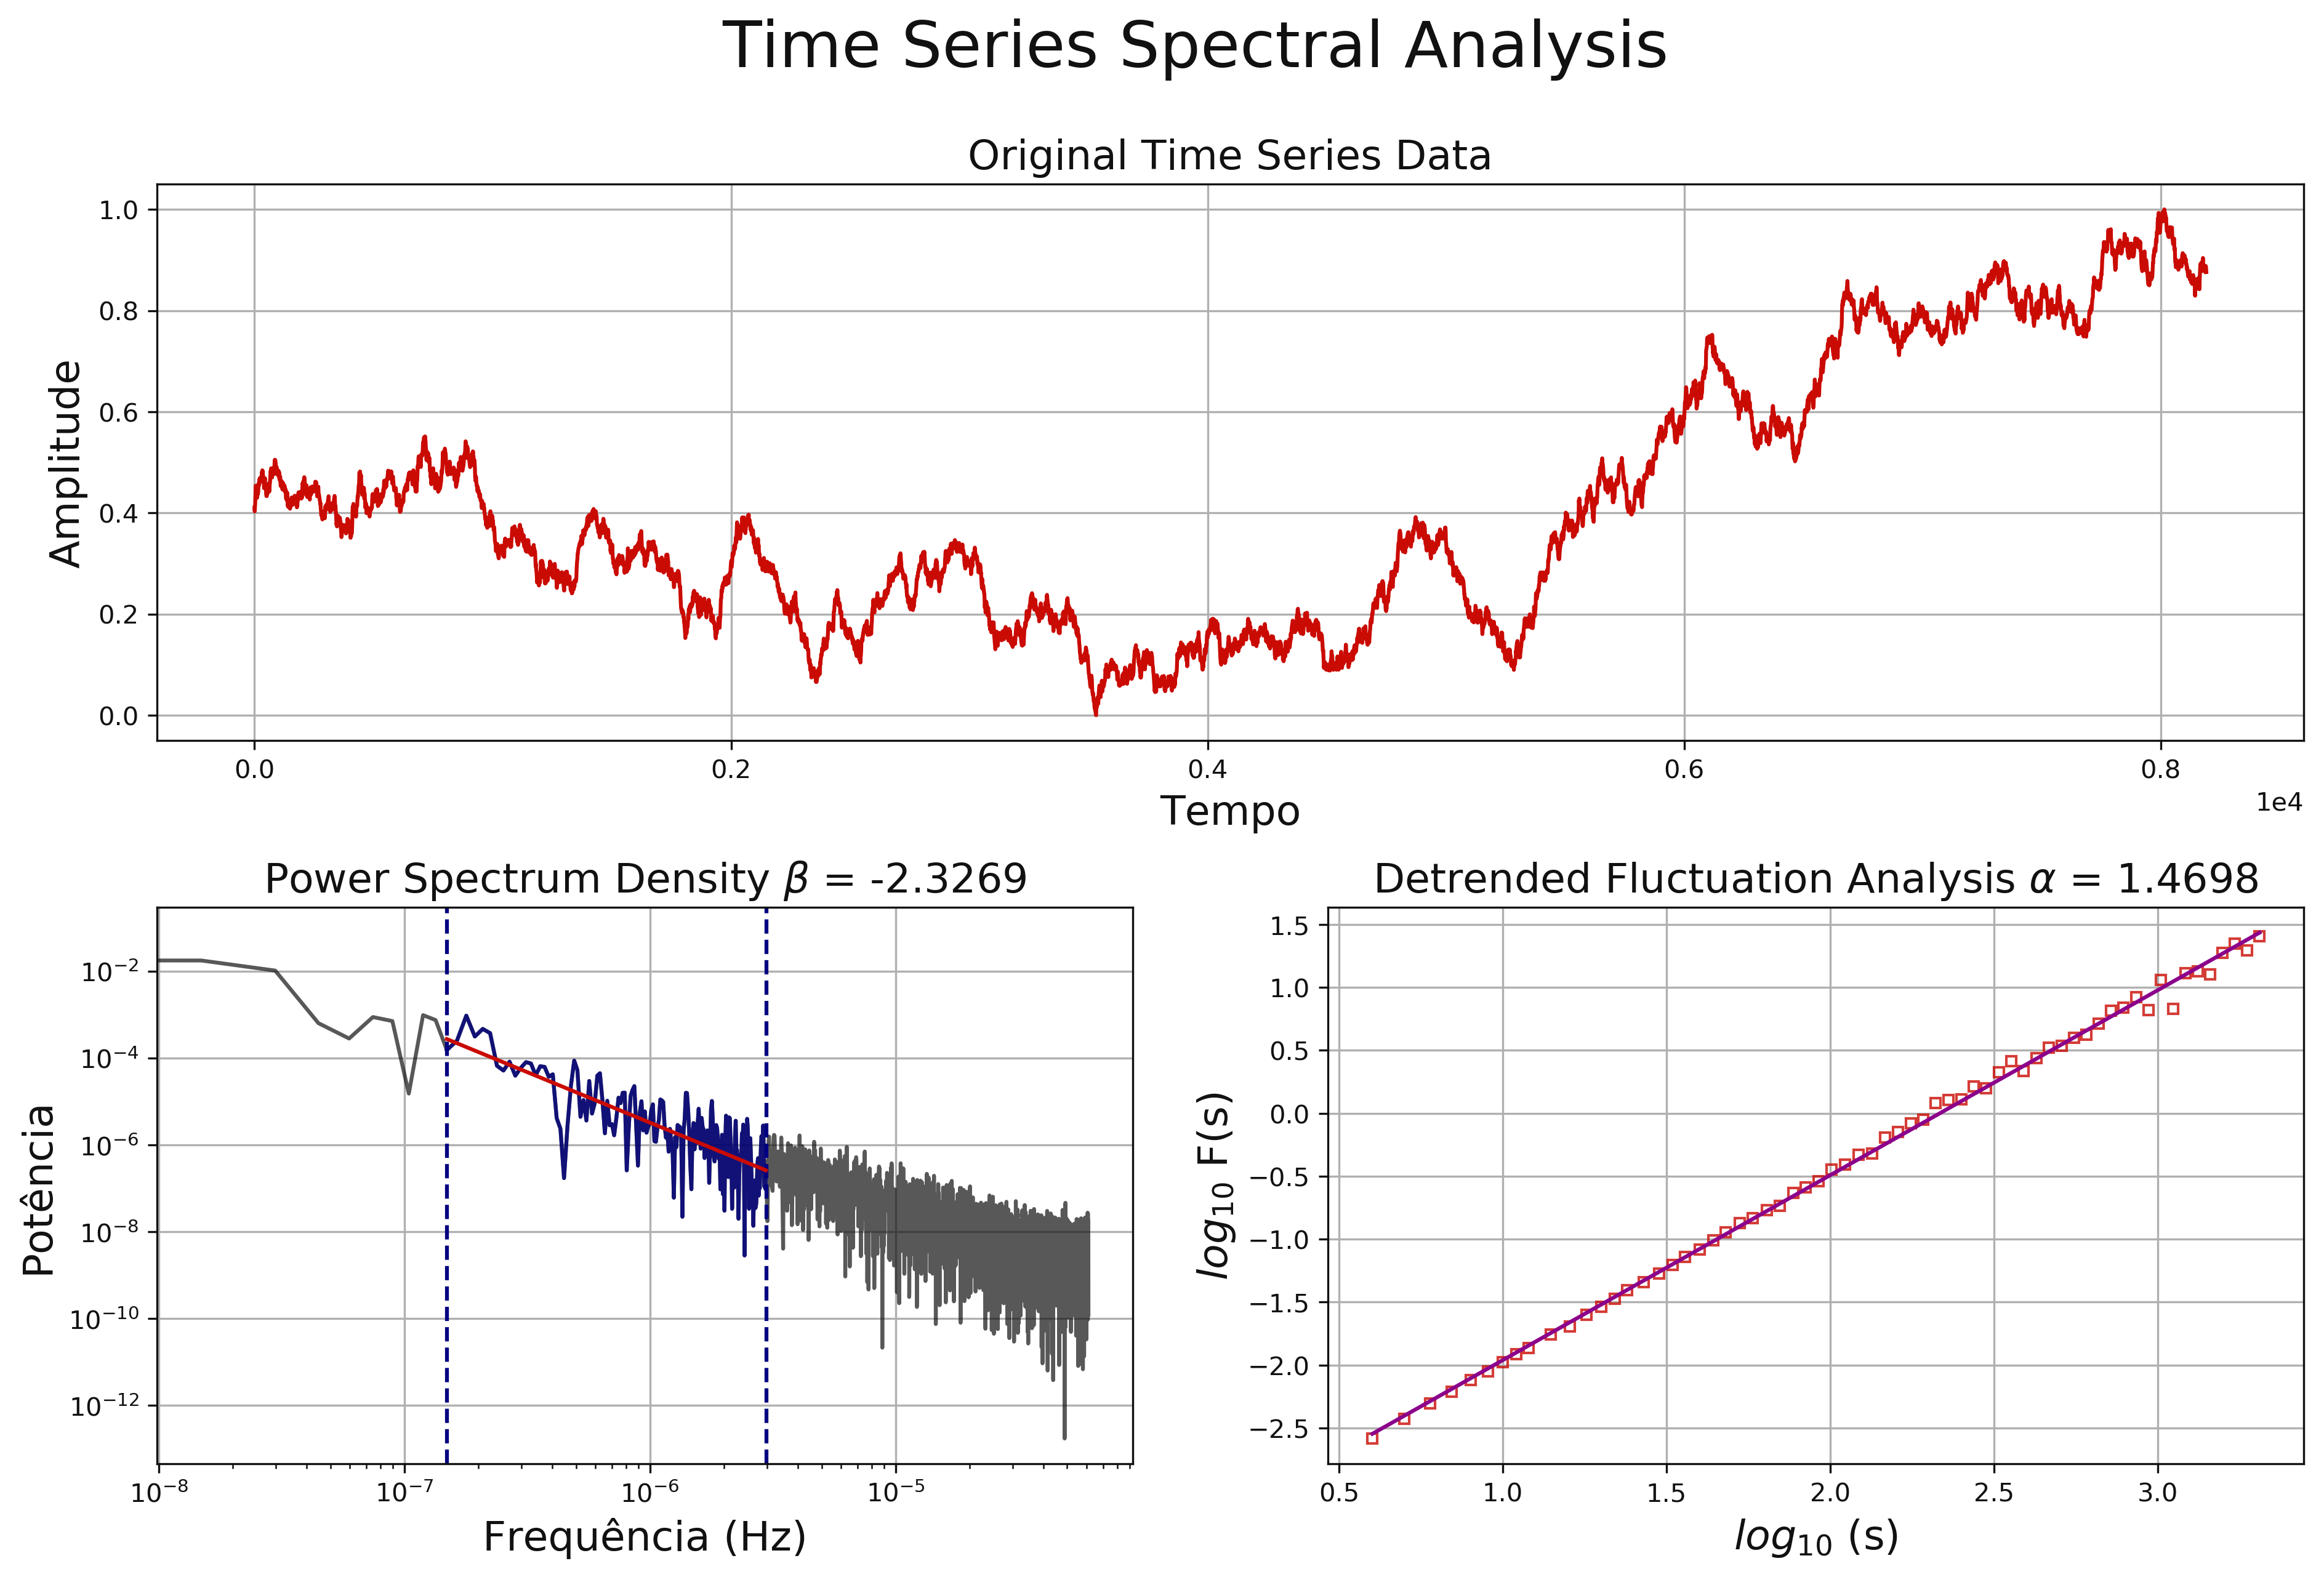
\includegraphics{Figuras/ex6/6_1/Exercicio6_1_grupo_noise_Specplus_n_8192.png}}		
	\end{center}
	\vspace{-2mm}	% acrescentar o espaçamento vertical apropriado entre a borda inferior da figura e a legenda ou a fonte quando não há legenda (o valor pode ser negativo para subir)
	\legenda{Figura 6.1.1: Acima, sinal do grupo noise com $n$ = 8192; abaixo à esquerda, o PSD e o índice espectral $\beta \sim$ -2.32; abaixo à direita, o DFA com o expoente $\alpha \sim$ 1.47.}	% legenda - para deixar sem legenda usar comando \legenda{} (nunca deve-se comentar o comando \legenda)
	\label{ex6_fig1}
	%\FONTE{}	% fonte consultada (elemento obrigatório, mesmo que seja produção do próprio autor)
\end{figure}

\begin{figure}[ht!]
	%\caption{Série e histogramas.}
	\vspace{-3mm}	% acrescentar o espaçamento vertical apropriado entre o título e a borda superior da figura
	\begin{center}
		\resizebox{8cm}{!}{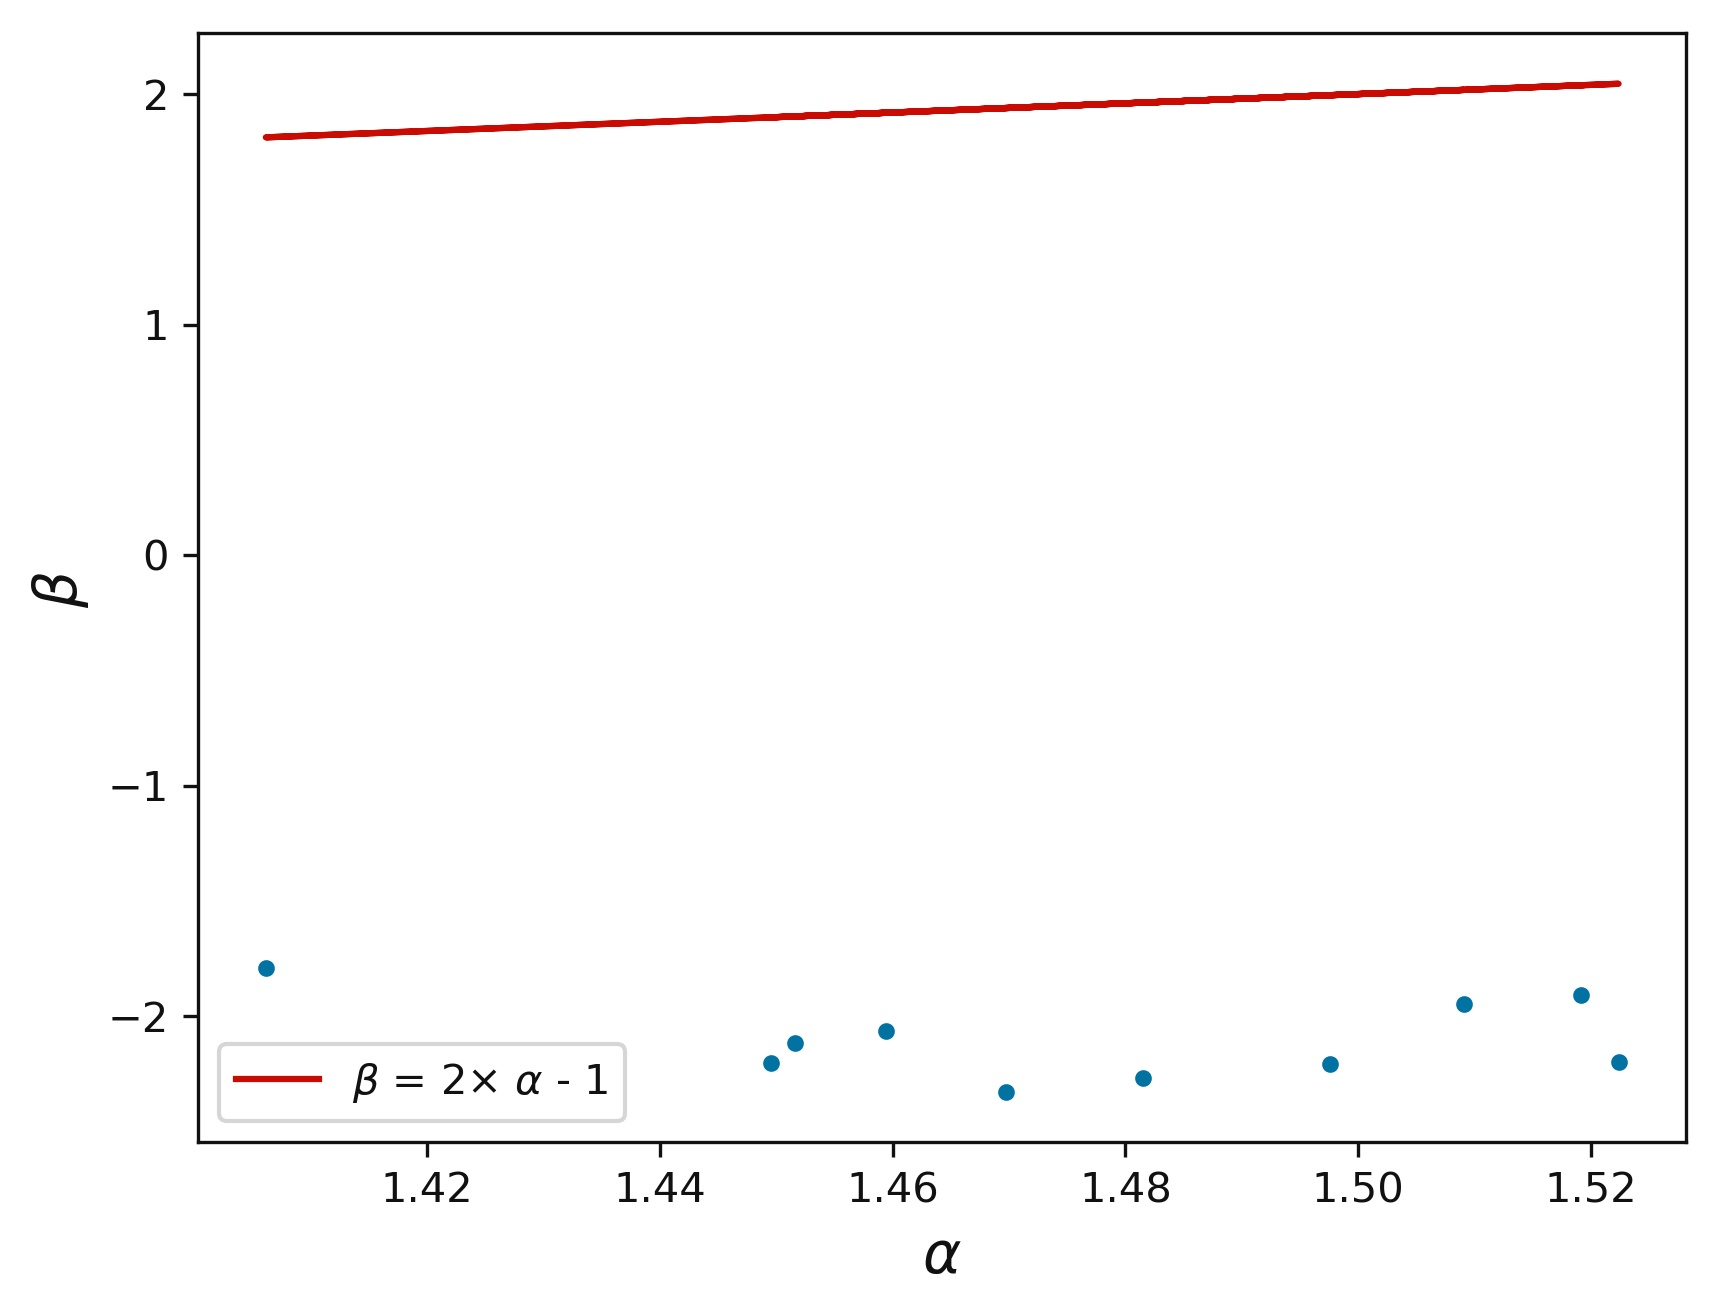
\includegraphics{Figuras/ex6/6_1/Exercicio6_1_grupo_noise_alfa_vs_beta_n_8192.jpg}}		
	\end{center}
	\vspace{-3mm}	% acrescentar o espaçamento vertical apropriado entre a borda inferior da figura e a legenda ou a fonte quando não há legenda (o valor pode ser negativo para subir)
	\legenda{Figura 6.1.2: Resultado do teste do ajuste dos valores de $\beta$ e $\alpha$ para a família noise com $n$ = 8192 à equação do Teorema de Wiener–Khinchin-Parseval. Os pontos são valores empíricos. A reta é o resultado da equação do Teorema de WKP sobre os $\alpha$'s empíricos. Observa-se que, em módulo, o $\beta$ teórico é compatível com o empírico.}	% legenda - para deixar sem legenda usar comando \legenda{} (nunca deve-se comentar o comando \legenda)
	\label{ex6_fig2}
	%\FONTE{}	% fonte consultada (elemento obrigatório, mesmo que seja produção do próprio autor)
\end{figure}

\clearpage
Primeiro resultado do agrupamento kmeans do grupo noise (usando $\beta$):

\begin{figure}[ht!]
	%\caption{Série e histogramas.}
	\vspace{-3mm}	% acrescentar o espaçamento vertical apropriado entre o título e a borda superior da figura
	\begin{center}
		\resizebox{14cm}{!}{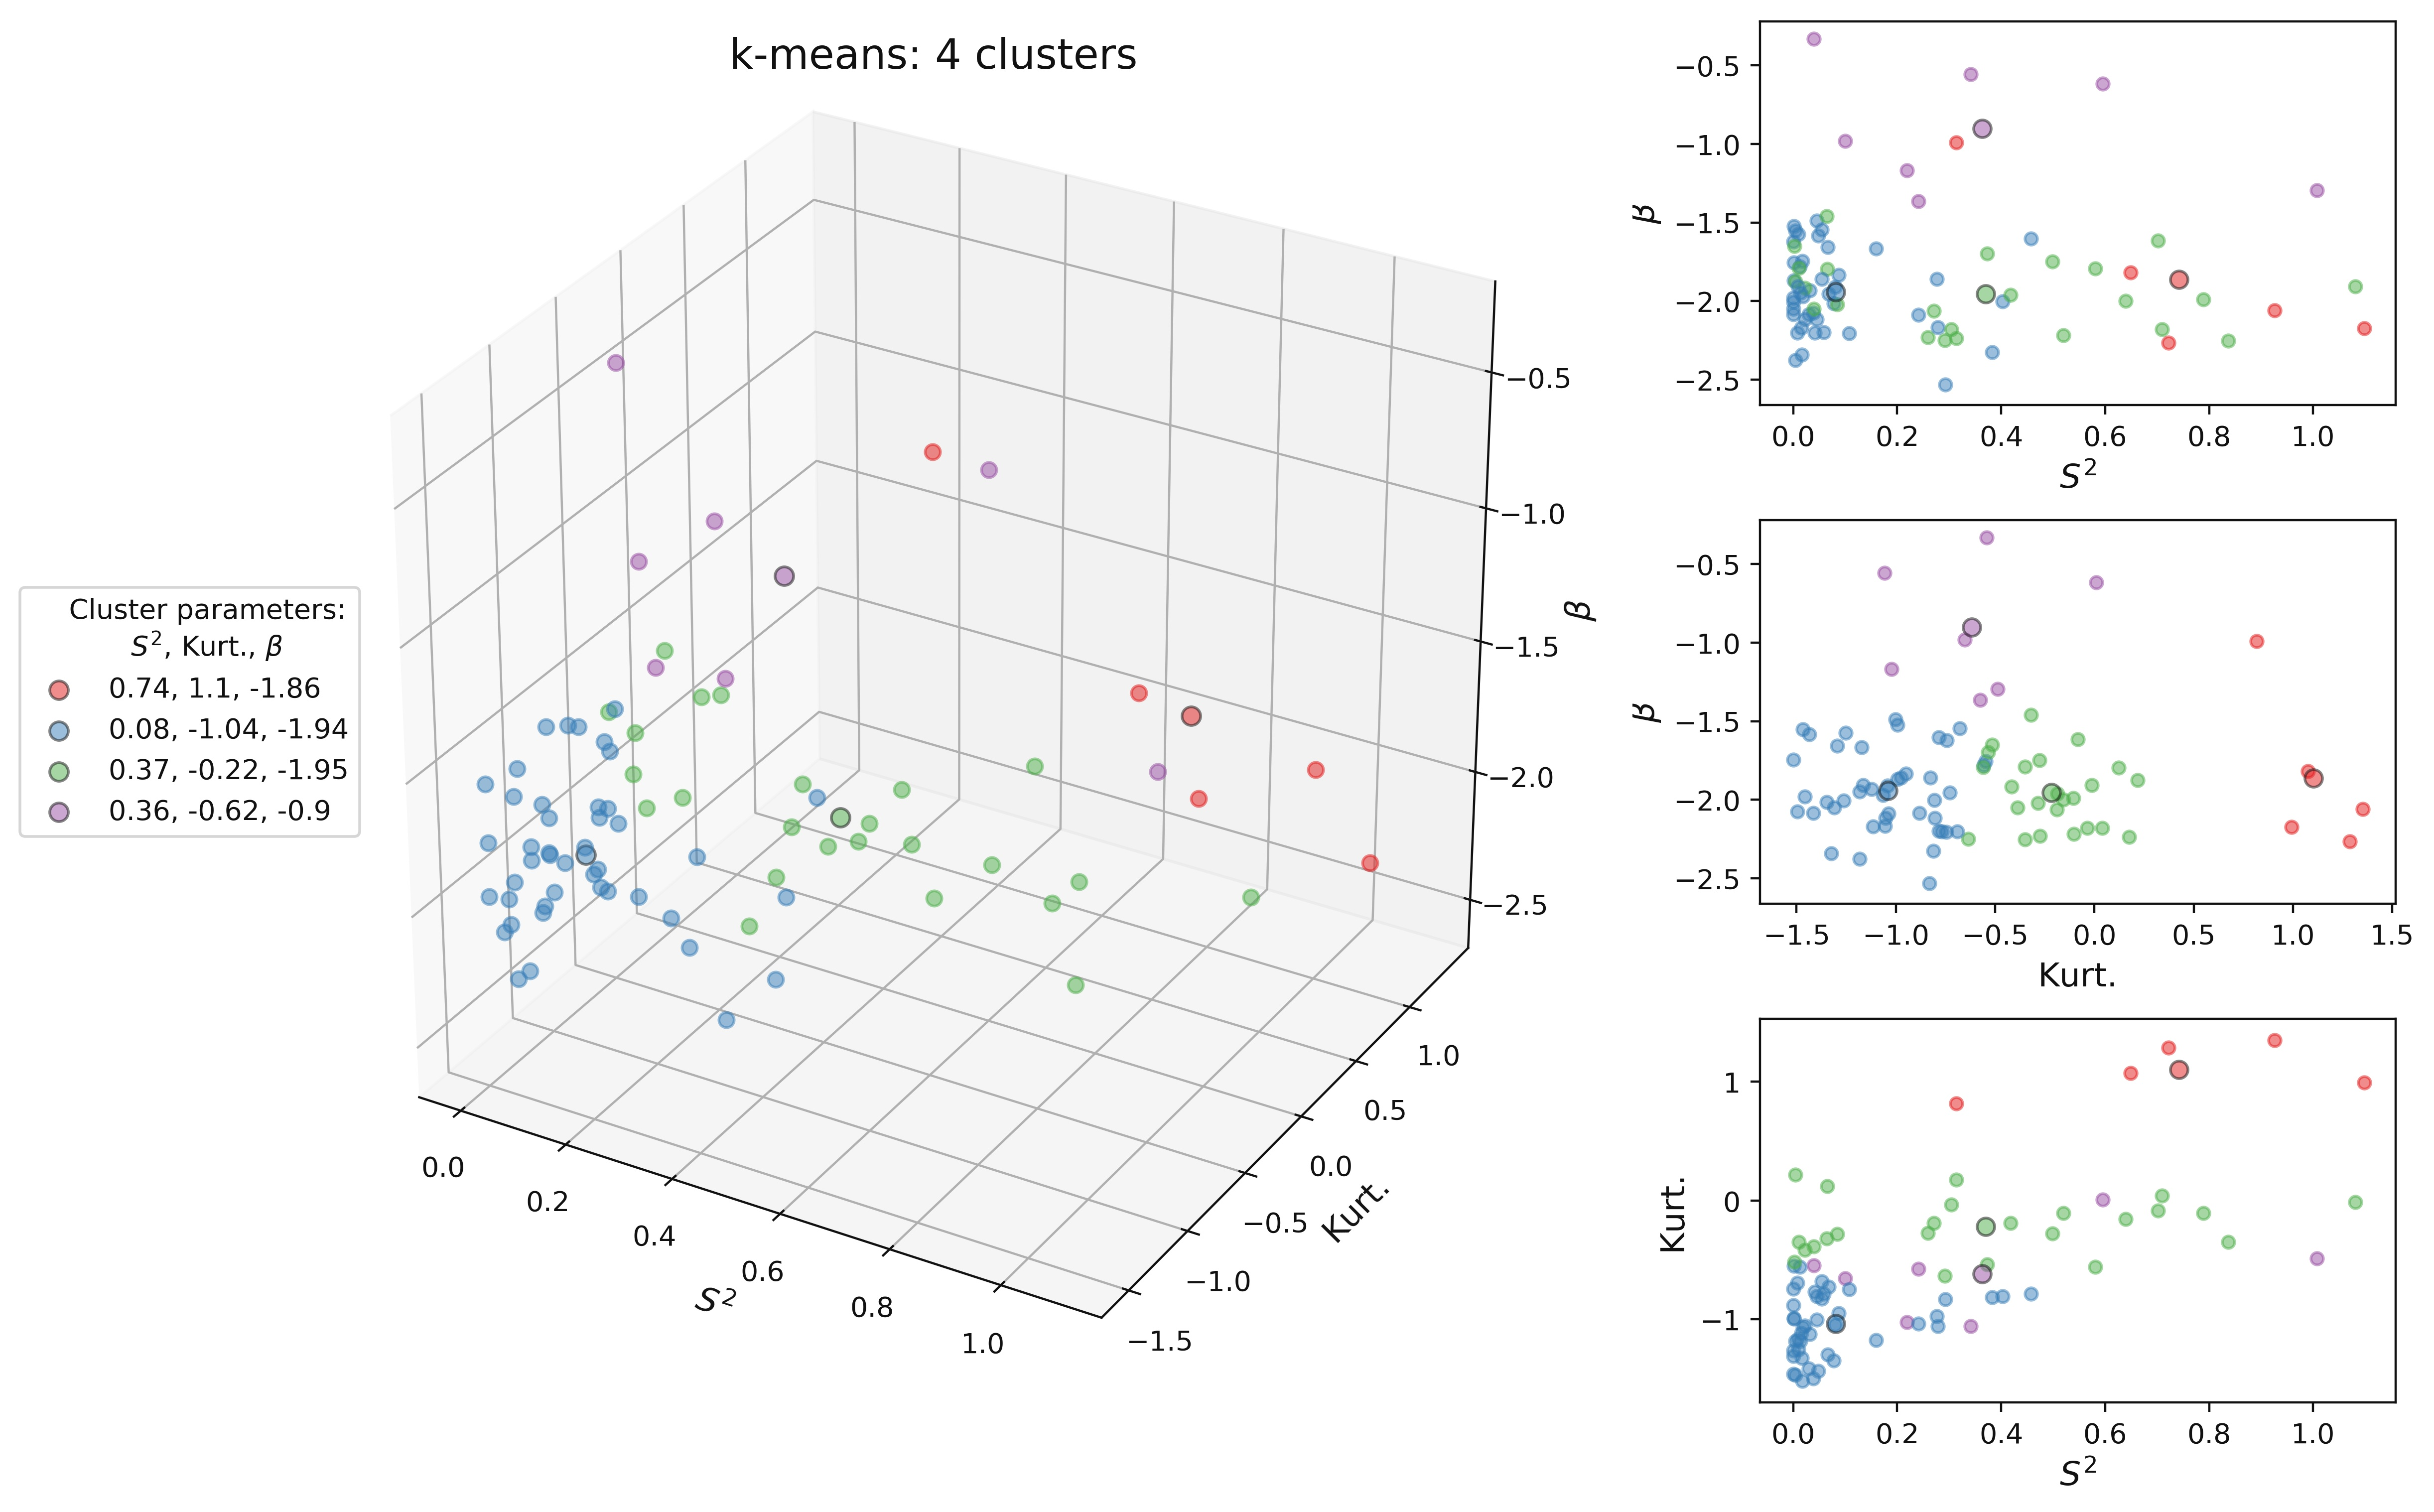
\includegraphics{Figuras/ex6/6_1/Exercicio6_1_grupo_noise_PSD_cluster_4.jpg}}		
	\end{center}
	\vspace{-3mm}	% acrescentar o espaçamento vertical apropriado entre a borda inferior da figura e a legenda ou a fonte quando não há legenda (o valor pode ser negativo para subir)
	\legenda{Figura 6.1.3: Técnica kmeans no espaço de parâmetros skewness$^{2}$ x kurtosis x $\beta$ para toda a família noise, cujo melhor resultado foi $n\_c$ = 4 (quatro clusters).}	% legenda - para deixar sem legenda usar comando \legenda{} (nunca deve-se comentar o comando \legenda)
	\label{ex6_fig3}
	%\FONTE{}	% fonte consultada (elemento obrigatório, mesmo que seja produção do próprio autor)
\end{figure}

Segundo resultado do agrupamento kmeans do grupo noise (usando $\alpha$):

\begin{figure}[ht!]
	%\caption{Série e histogramas.}
	\vspace{-3mm}	% acrescentar o espaçamento vertical apropriado entre o título e a borda superior da figura
	\begin{center}
		\resizebox{14cm}{!}{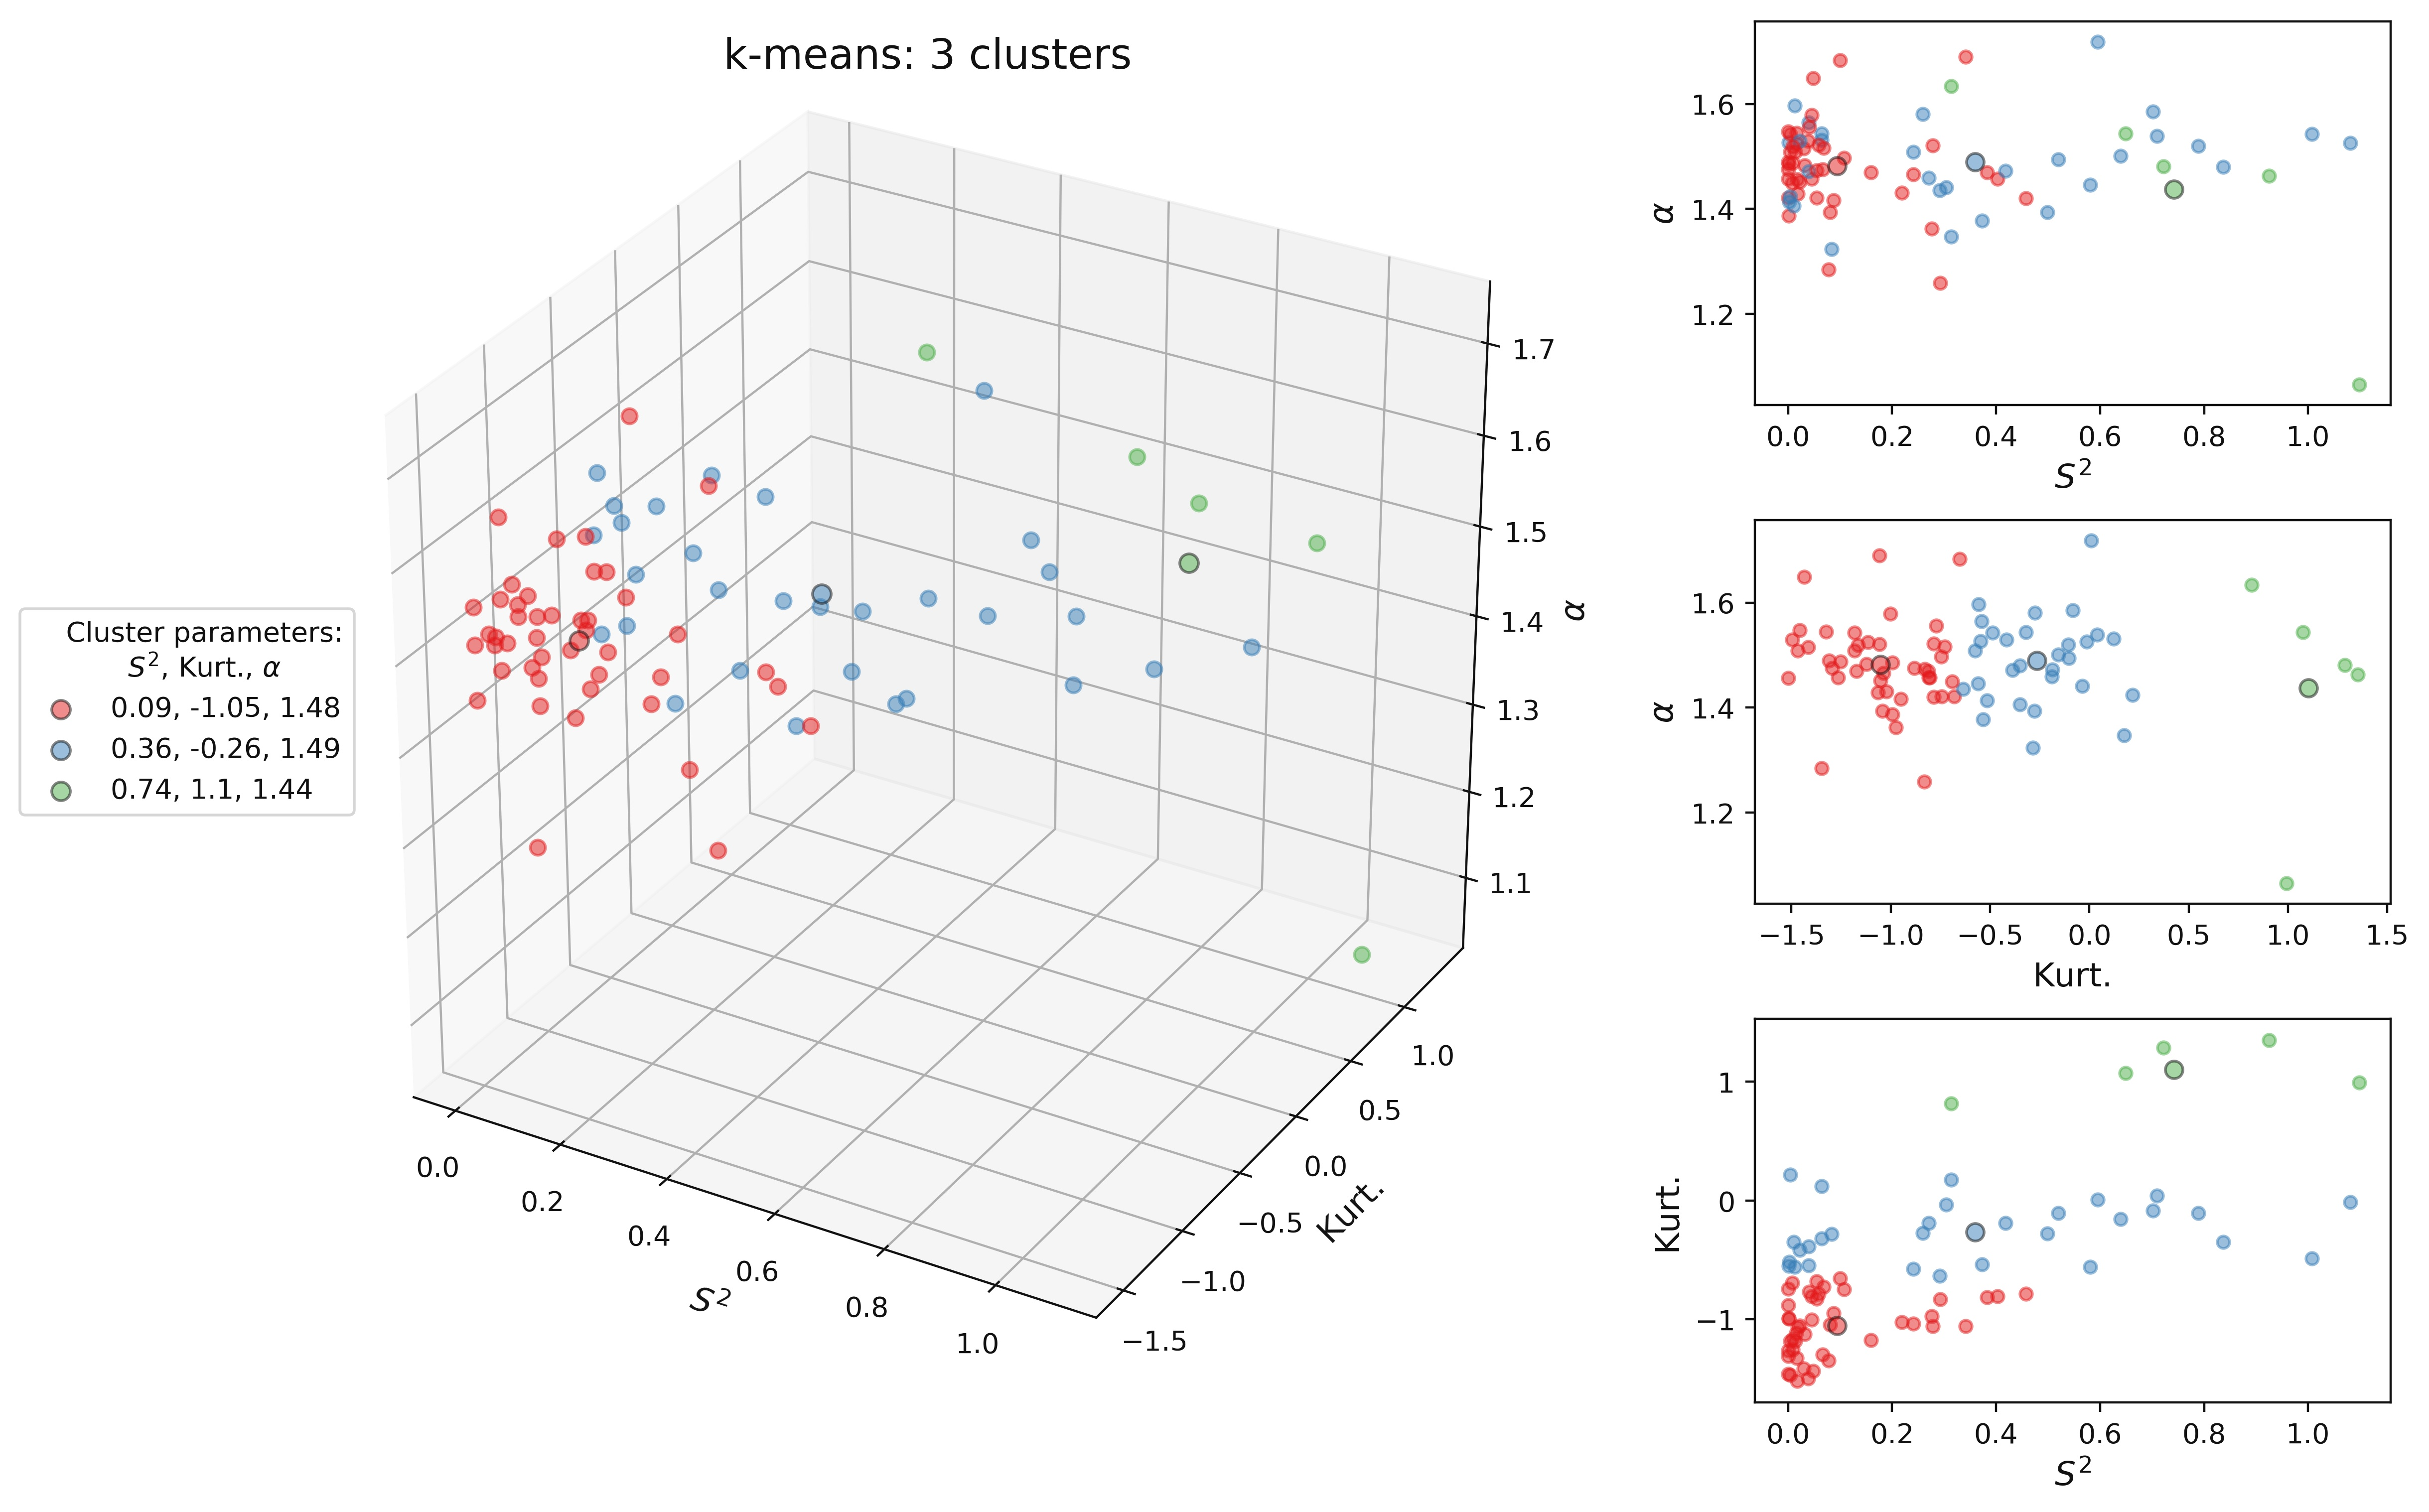
\includegraphics{Figuras/ex6/6_1/Exercicio6_1_grupo_noise_DFA_cluster_3.jpg}}		
	\end{center}
	\vspace{-3mm}	% acrescentar o espaçamento vertical apropriado entre a borda inferior da figura e a legenda ou a fonte quando não há legenda (o valor pode ser negativo para subir)
	\legenda{Figura 6.1.4: Técnica kmeans no espaço de parâmetros skewness$^{2}$ x kurtosis x $\alpha$ para toda a família noise, cujo melhor resultado foi $n\_c$ = 3 (três clusters).}	% legenda - para deixar sem legenda usar comando \legenda{} (nunca deve-se comentar o comando \legenda)
	\label{ex6_fig3}
	%\FONTE{}	% fonte consultada (elemento obrigatório, mesmo que seja produção do próprio autor)
\end{figure}

%%%%%%%%%%%%%%%%% Extra! %%%%%%%%%%%%%%%%%%%%%%%

\clearpage
Importante ressaltar que as análises espectrais do grupo colornoise foram consistentes com as cores de cada ruído ($\beta$ = 0, 1 e 2). A seguir está um plot da análise para $\beta$ = 1 (Figura 6.1.5). Por outro lado, a análise espectral do grupo chaosnoise apresentou índice espectral com faixa dinâmica extremamente ''lisa'', similar a um ruído branco. Isso ocorre pois as séries do grupo chaosnoise, como o mapeamento Logístico (Figura 6.1.6), pertencem a regimes antipersistentes. 

\begin{figure}[ht!]
	%\caption{Série e histogramas.}
	\vspace{-4mm}	% acrescentar o espaçamento vertical apropriado entre o título e a borda superior da figura
	\begin{center}
		\resizebox{12cm}{!}{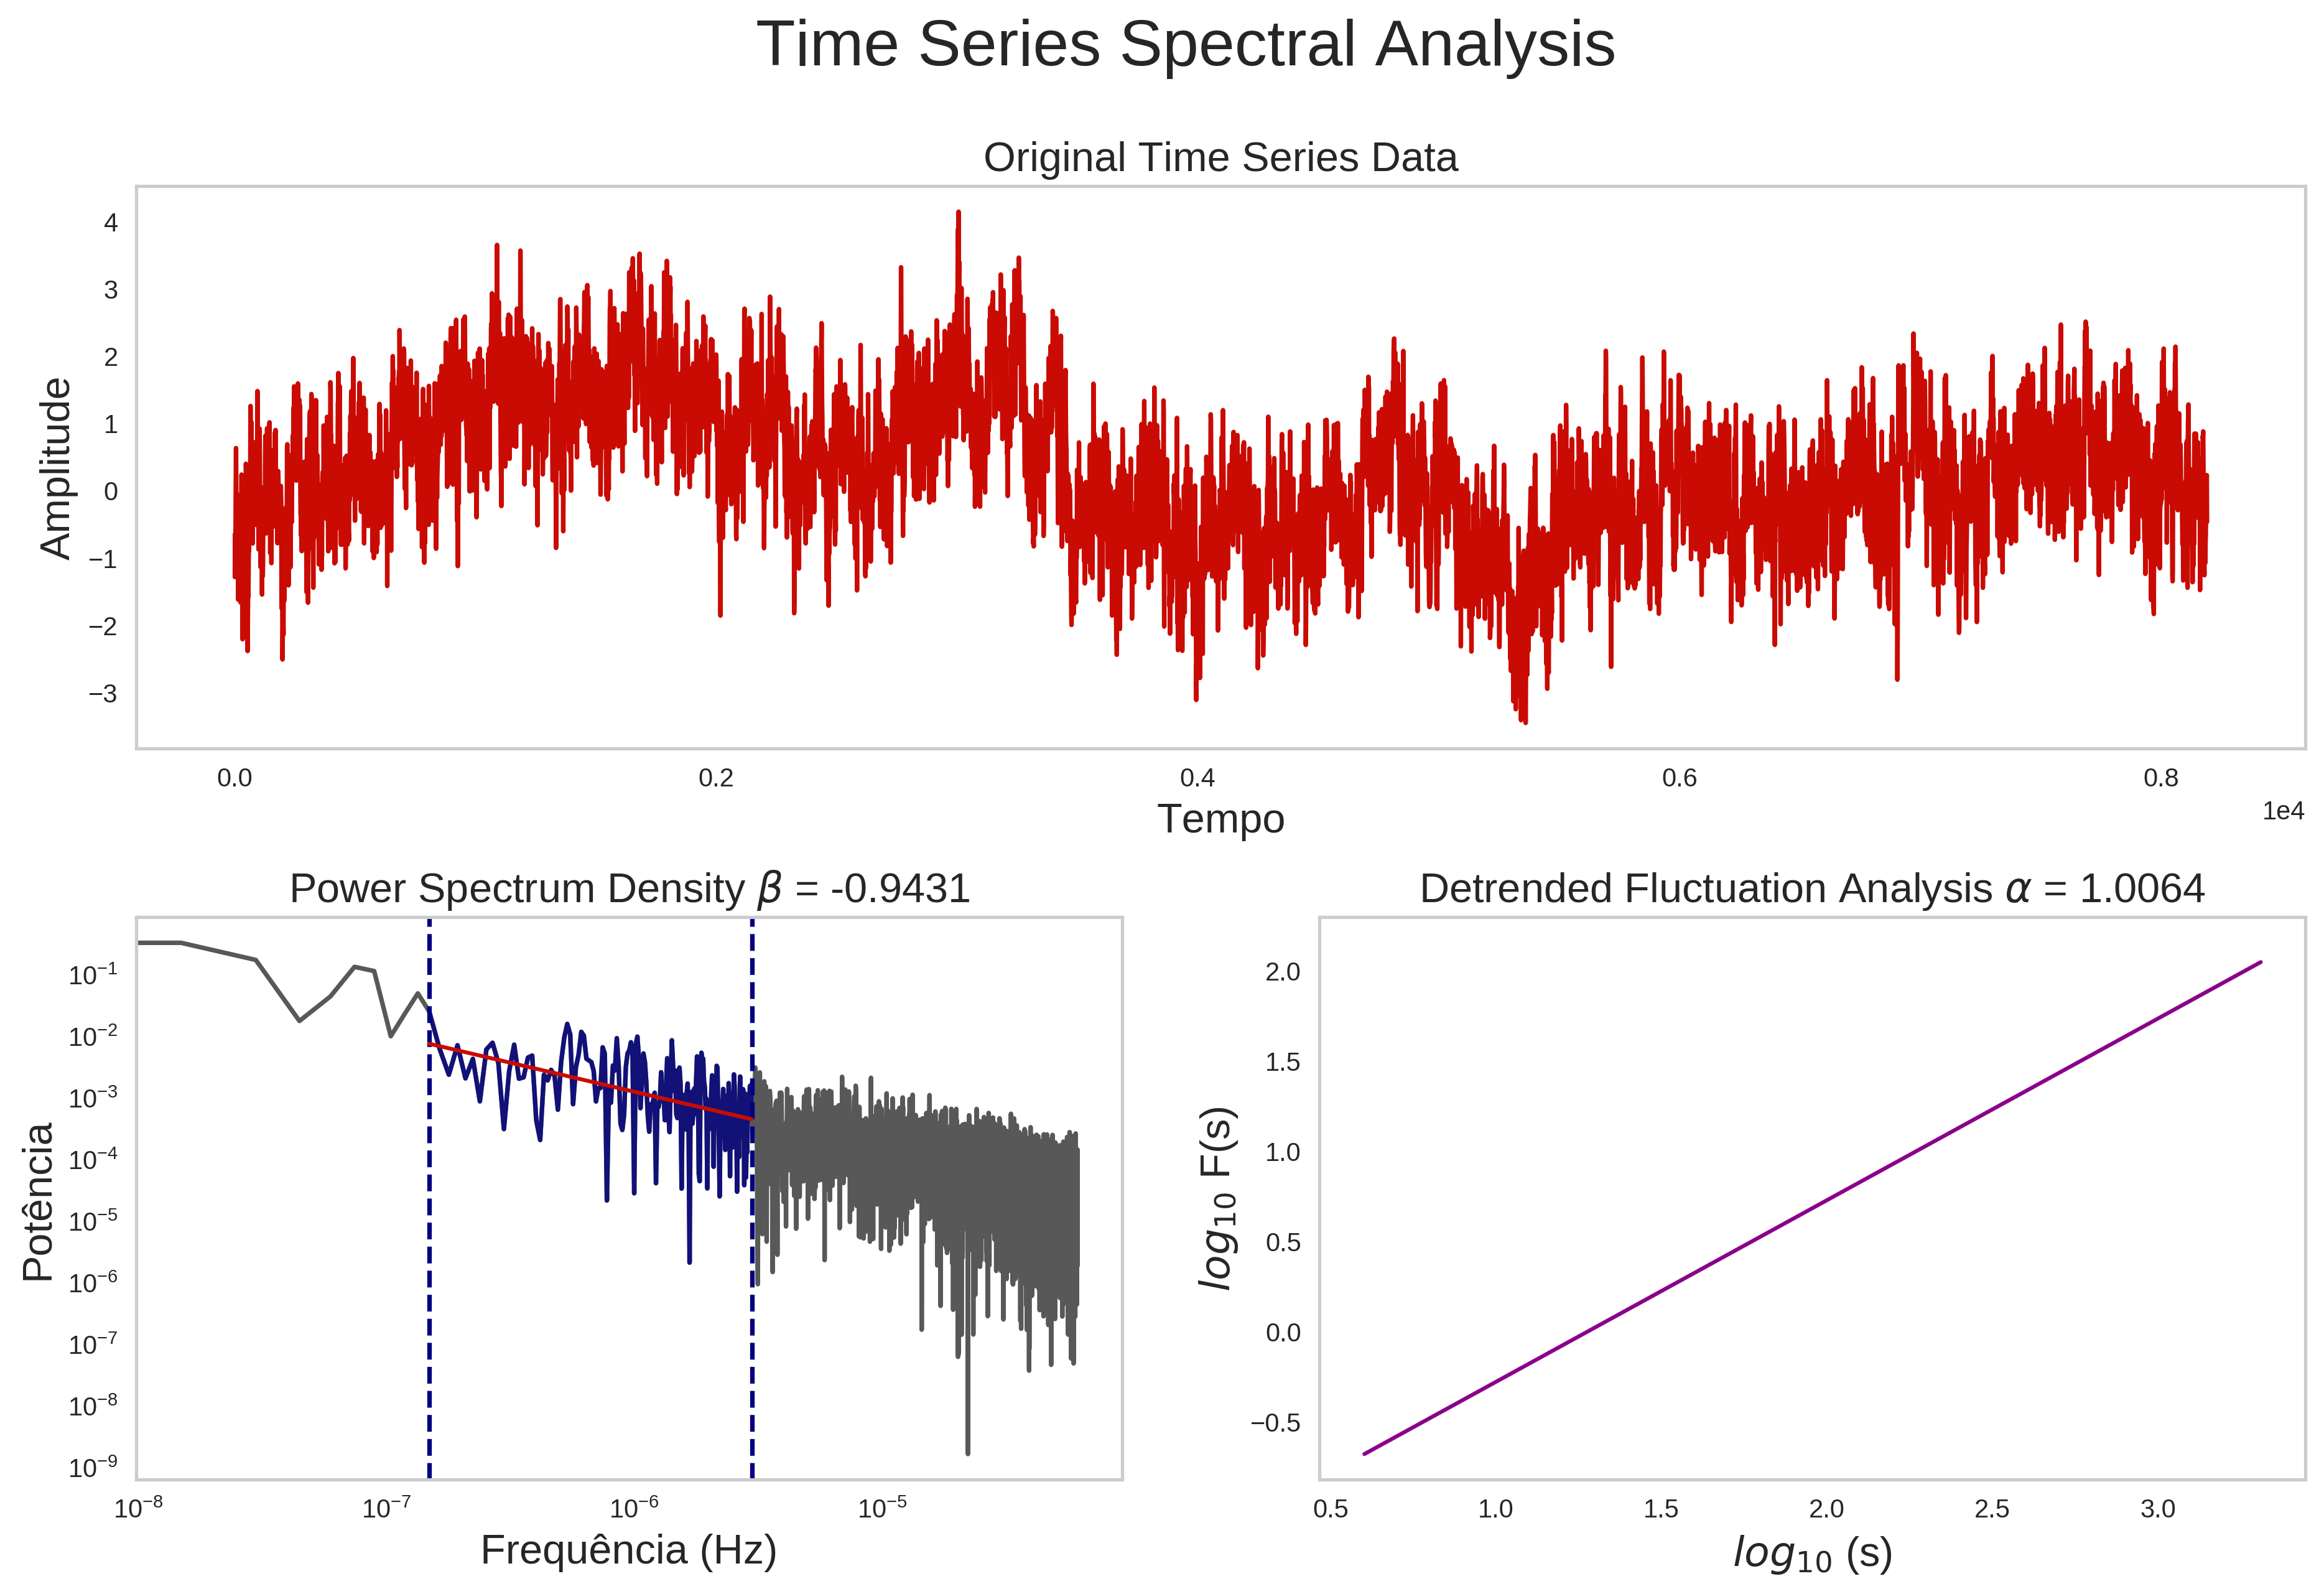
\includegraphics{Figuras/ex6/6_1/Exercicio6_1_grupo_colornoise_Specplus_betaNoise_1_ANALYSIS_PSD_DFA_2.png}}		
	\end{center}
	\vspace{-2mm}	% acrescentar o espaçamento vertical apropriado entre a borda inferior da figura e a legenda ou a fonte quando não há legenda (o valor pode ser negativo para subir)
	\legenda{Figura 6.1.5: Análise espectral do grupo colornoise para $\beta$ = 1.}	% legenda - para deixar sem legenda usar comando \legenda{} (nunca deve-se comentar o comando \legenda)
	\label{ex6_fig1}
	%\FONTE{}	% fonte consultada (elemento obrigatório, mesmo que seja produção do próprio autor)
\end{figure}

\begin{figure}[ht!]
	%\caption{Série e histogramas.}
	\vspace{-4mm}	% acrescentar o espaçamento vertical apropriado entre o título e a borda superior da figura
	\begin{center}
		\resizebox{12cm}{!}{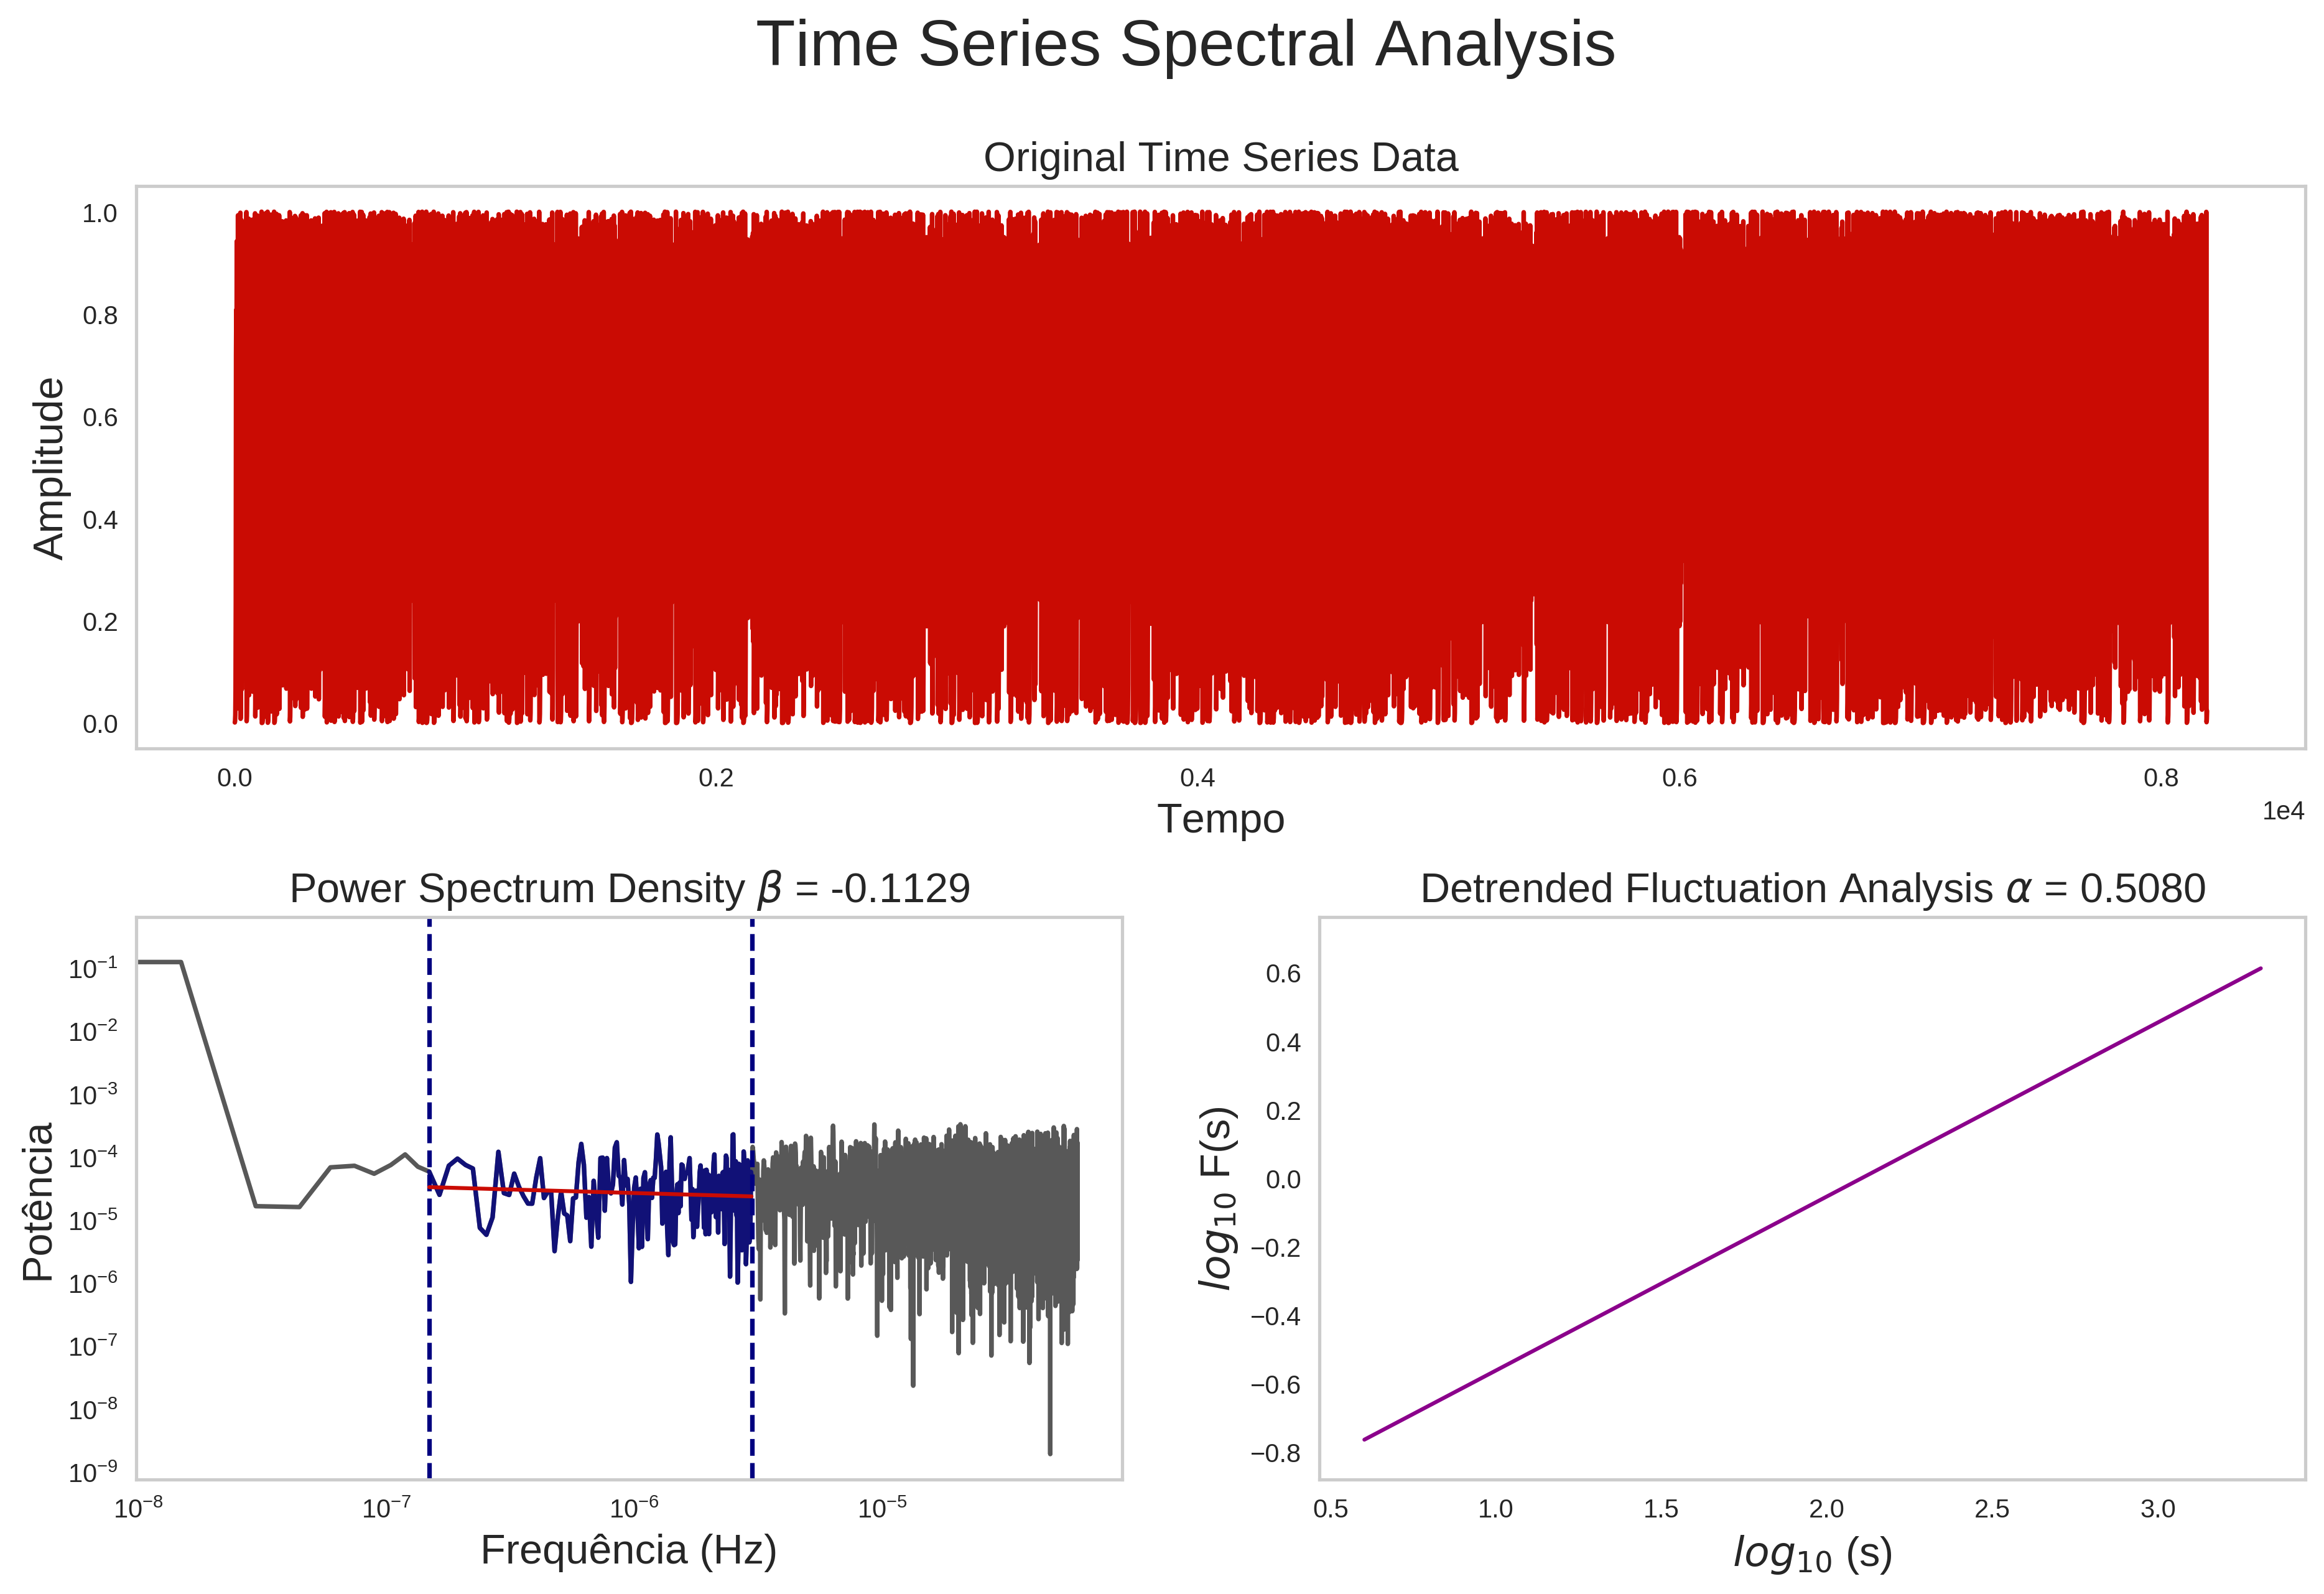
\includegraphics{Figuras/ex6/6_1/Exercicio6_1_Logistico_Specplus_rho_4.0_ANALYSIS_PSD_DFA_2.png}}		
	\end{center}
	\vspace{-2mm}	% acrescentar o espaçamento vertical apropriado entre a borda inferior da figura e a legenda ou a fonte quando não há legenda (o valor pode ser negativo para subir)
	\legenda{Figura 6.1.6: Análise espectral do grupo chaosnoise para o mapeamento Logístico com $\rho$ = 4.}	% legenda - para deixar sem legenda usar comando \legenda{} (nunca deve-se comentar o comando \legenda)
	\label{ex6_fig1}
	%\FONTE{}	% fonte consultada (elemento obrigatório, mesmo que seja produção do próprio autor)
\end{figure}

%%%%%%%%%%%%%%%%%%%%%%%%%%%%%%%%%%%%5 6.2 %%%%%%%%%%%%%%%%%%%%%%%%%%%%%%%%%%%%%%%%%%%%%
\clearpage
\subsection*{6.2}
\addcontentsline{toc}{section}{\protect\numberline{} 6.2}%

%Os plots a seguir exemplificam a análise realizada. 
Para este exercício foi utilizado o script kmeans\_3D\_plus\_data.py. Os resultados de cada família estão em suas respectivas pastas dentro da pasta referente a este exercício - \textbf{6.2}. As séries temporais \textit{ST-Sol3GHz} e \textit{ST-surftemp504} foram importadas da pasta \textbf{time\_series\_data}. A \textit{ST-OWS\_NDC\_Covid19} é referente ao Brasil e foi baixada na execução do código. 

Os plots a seguir foram escolhidos por exibir os resultados mais interessantes. Cada família está identificada com a cor vermelha (representando um cluster único, ou seja, $n\_c$ = 1) e as séries temporais acima citadas são plotadas no mesmo espaço de parâmetros. Com isso pode-se identificar como as séries temporais se posicionam nos espaços considerados com relação aos sinais presentes na tabela \textit{Dataset\_signal}. De todas as famílias, apenas chaosnoise não permitiu identificar alguma das três séries temporais como pertencente ao cluster da família. Para o grupo noise (Figura 6.2.1), a série \textit{ST-surftemp504} esteve próxima dos sinais da família no espaço skewness$^{2}$ x kurtosis x $\beta$, mas nenhuma série temporal exibiu o mesmo comportamento no espaço skewness$^{2}$ x kurtosis x $\alpha$. Para os grupos colornoise (Figura 6.2.2) e pmnoise (Figura 6.2.3), o comportamento das séries temporais com relação aos sinais foi basicamente o mesmo para ambos os espaços de parâmetros considerados.

\begin{figure}[ht!]
	%\caption{Série e histogramas.}
	\vspace{0mm}	% acrescentar o espaçamento vertical apropriado entre o título e a borda superior da figura
	\begin{center}
		\resizebox{14cm}{!}{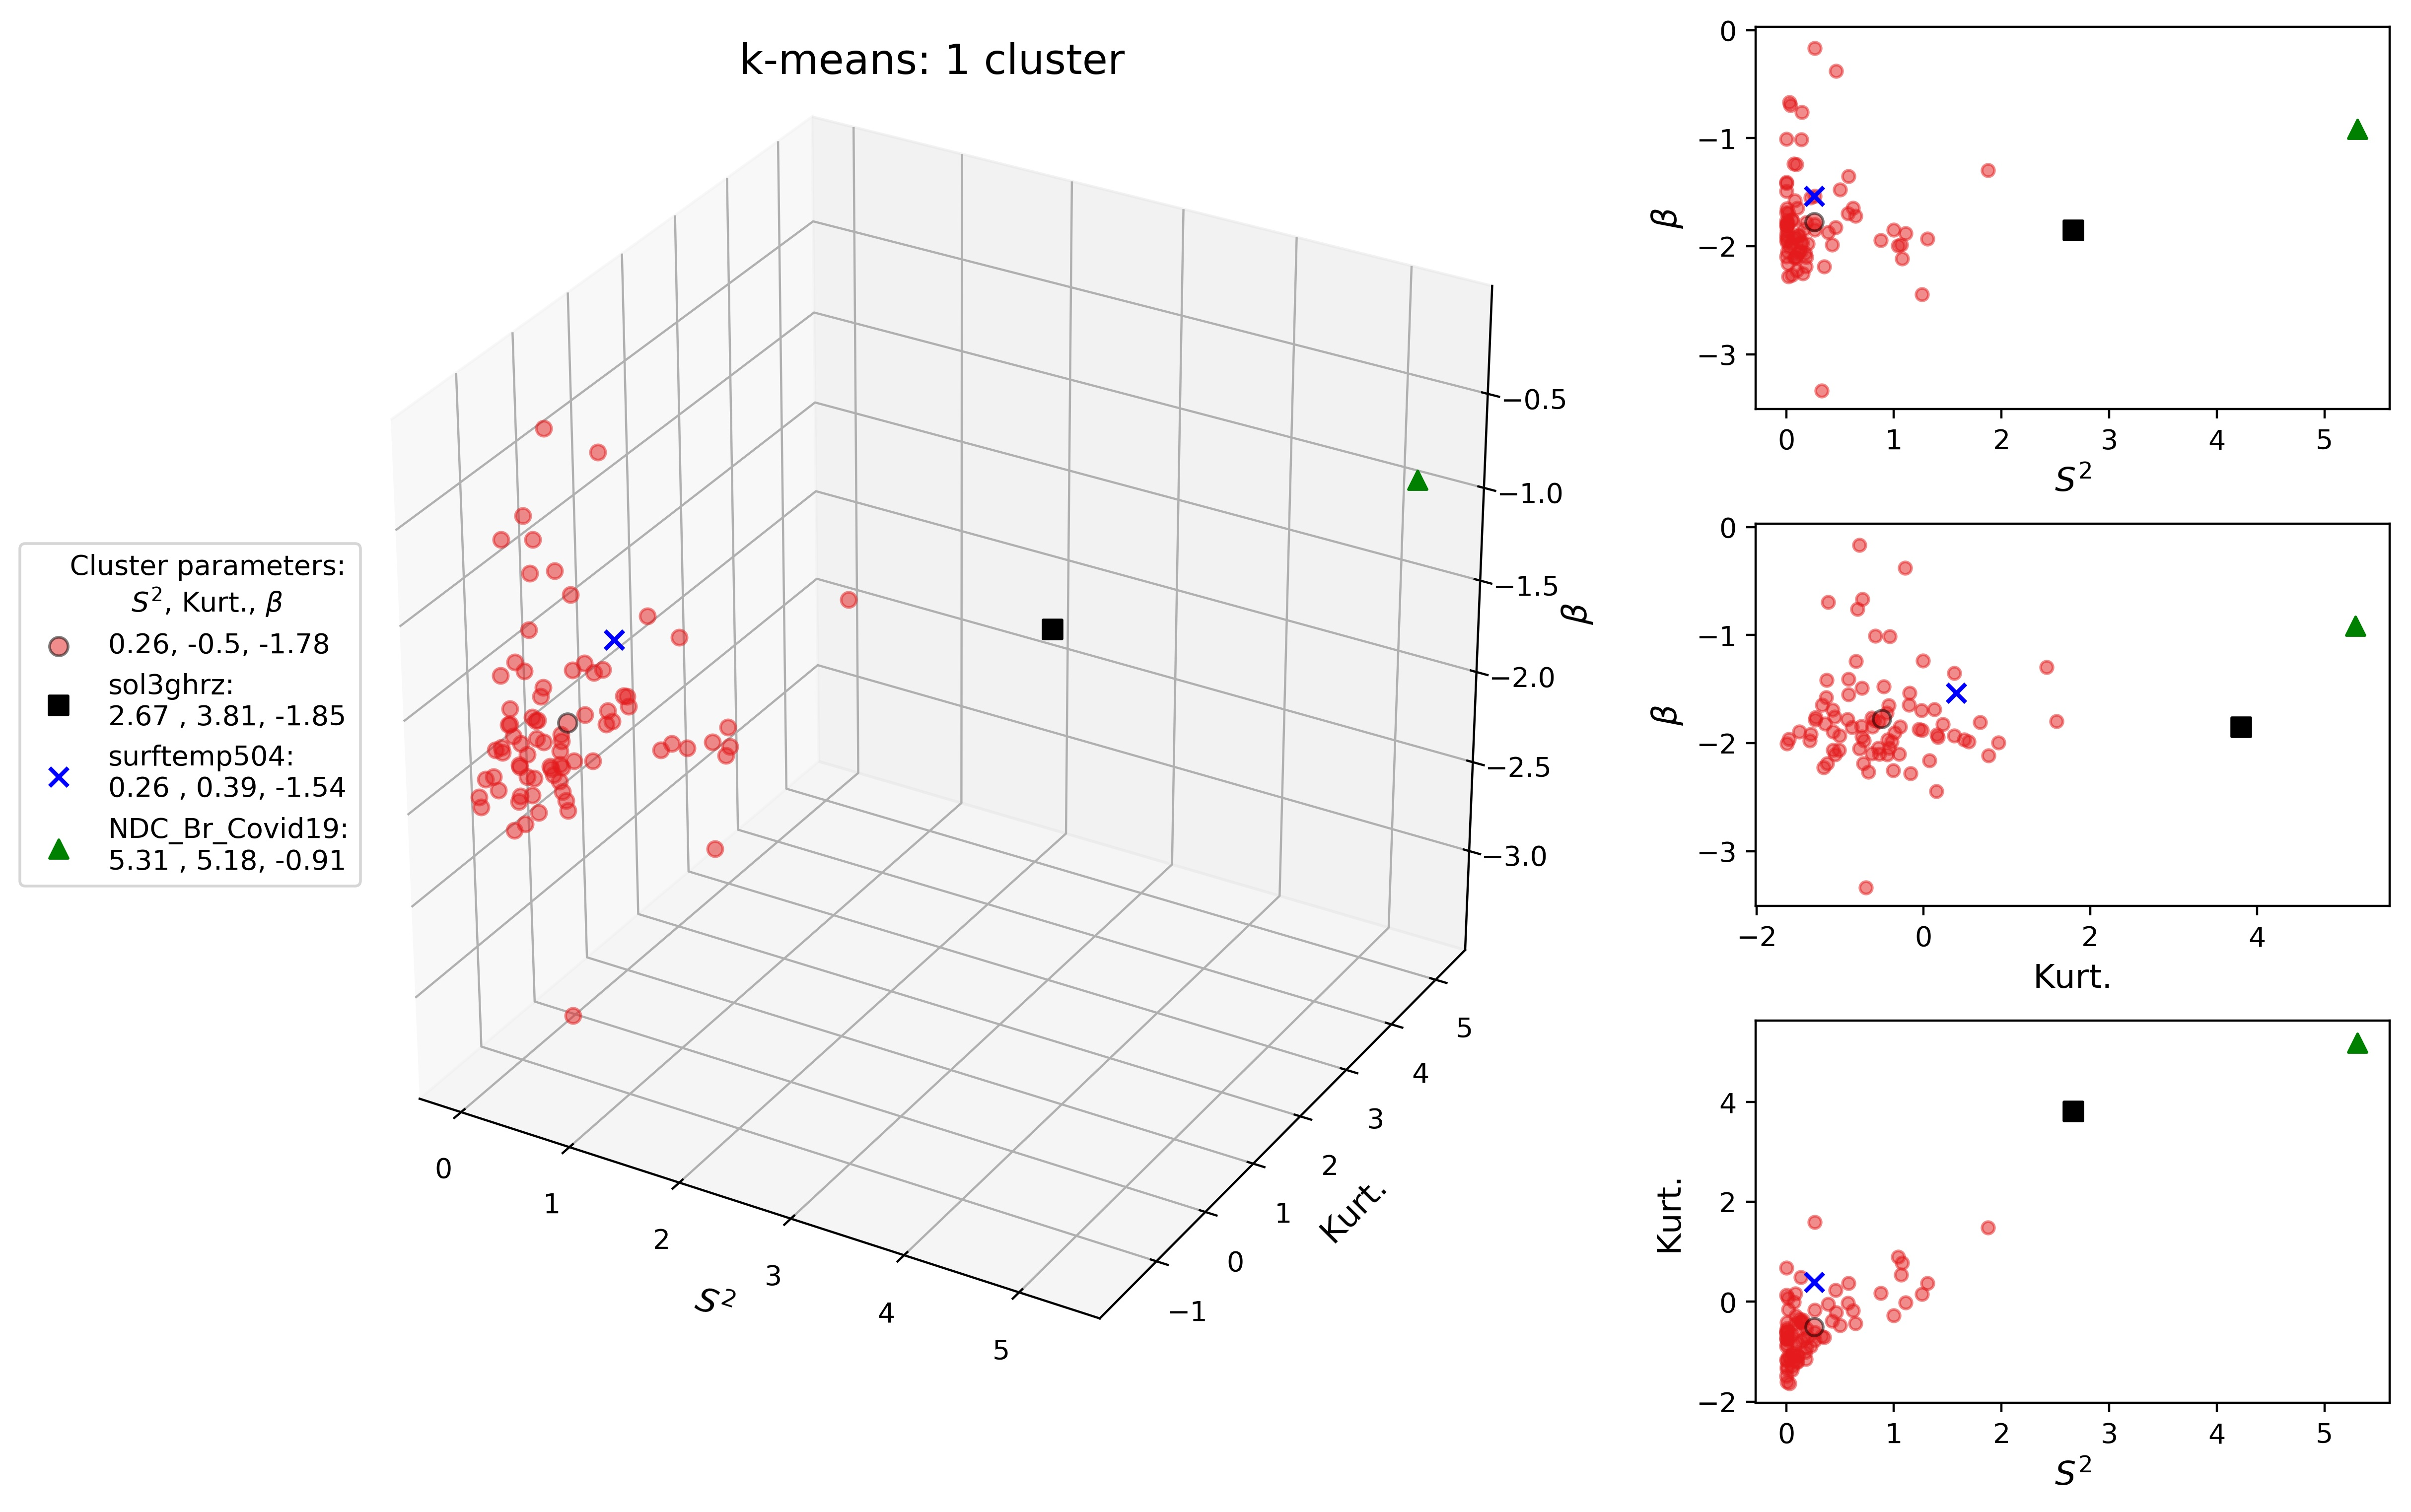
\includegraphics{Figuras/ex6/6_2/Exercicio6_2_grupo_noise_PSD_cluster_1.jpg}}		
	\end{center}
	\vspace{-2mm}	% acrescentar o espaçamento vertical apropriado entre a borda inferior da figura e a legenda ou a fonte quando não há legenda (o valor pode ser negativo para subir)
	\legenda{Figura 6.2.1: Espaço skewness$^{2}$ x kurtosis x $\beta$ do grupo noise e a posição relativa das três séries temporais deste exercício. A série \textit{ST-surftemp504} foi a que mais se aproximou dos sinais deste grupo.}	% legenda - para deixar sem legenda usar comando \legenda{} (nunca deve-se comentar o comando \legenda)
	\label{ex6_fig3}
	%\FONTE{}	% fonte consultada (elemento obrigatório, mesmo que seja produção do próprio autor)
\end{figure}

\begin{figure}[ht!]
	%\caption{Série e histogramas.}
	\vspace{0mm}	% acrescentar o espaçamento vertical apropriado entre o título e a borda superior da figura
	\begin{center}
		\resizebox{14cm}{!}{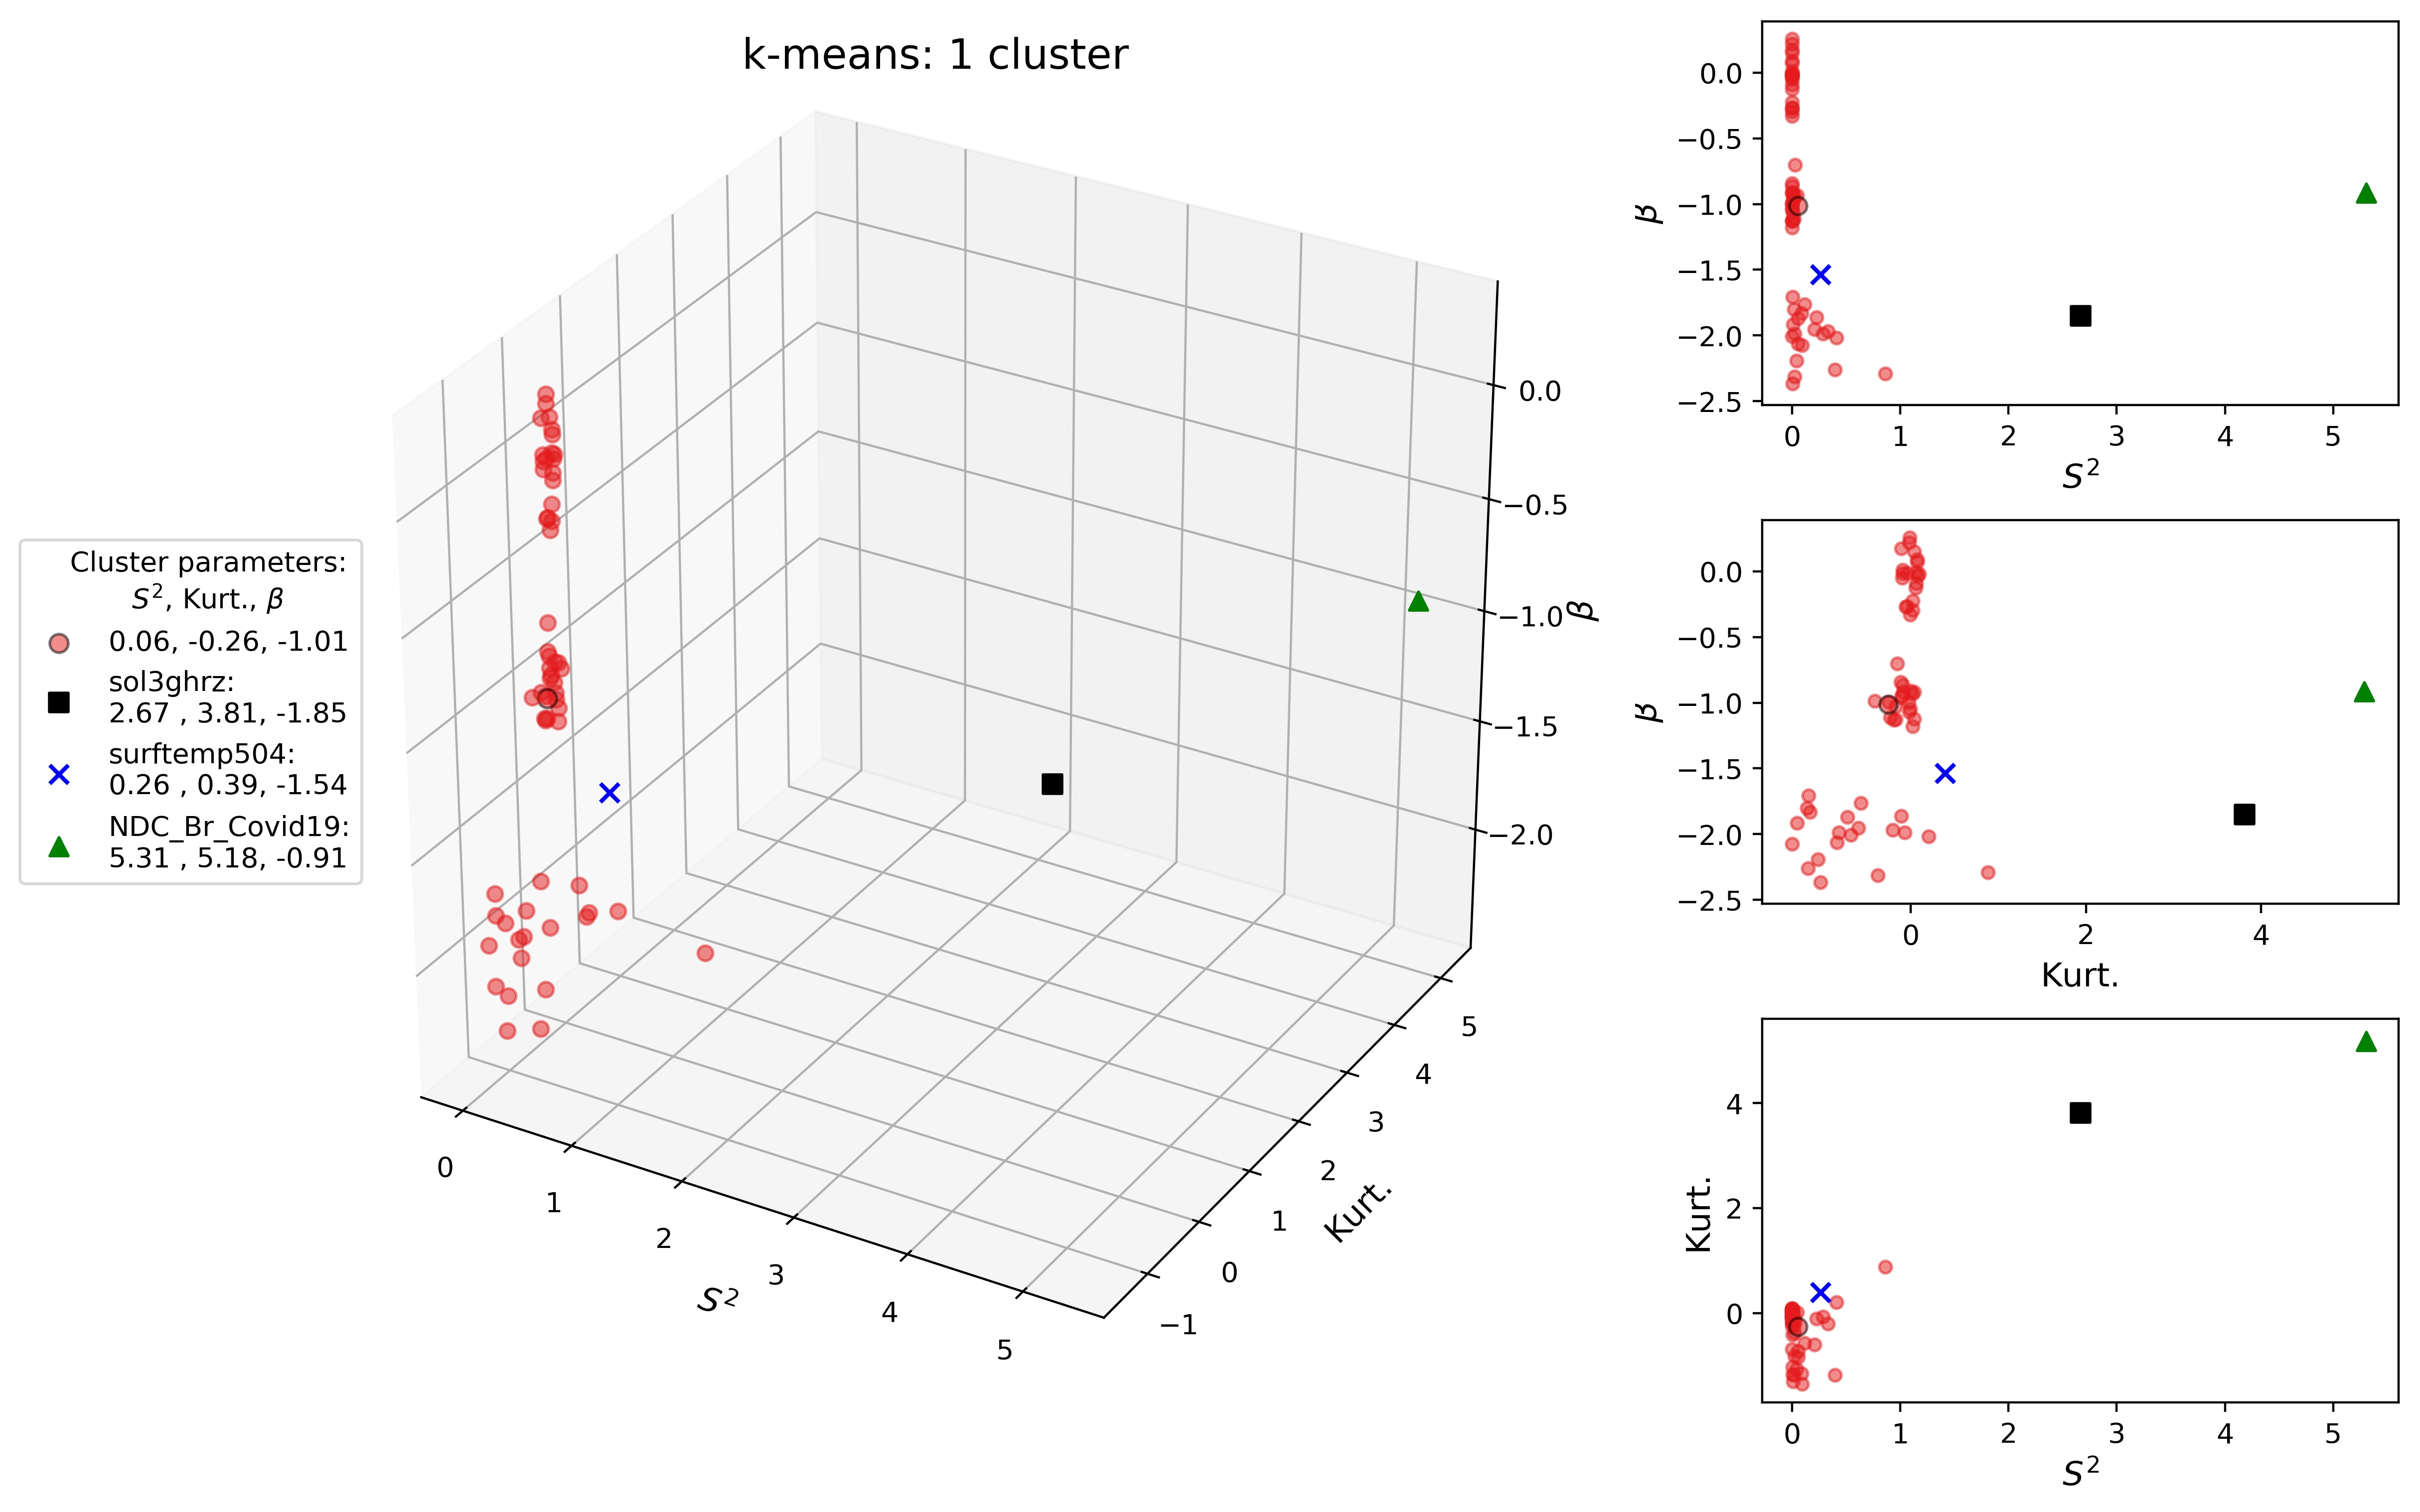
\includegraphics{Figuras/ex6/6_2/Exercicio6_2_grupo_colornoise_PSD_cluster_1.jpg}}		
	\end{center}
	\vspace{-2mm}	% acrescentar o espaçamento vertical apropriado entre a borda inferior da figura e a legenda ou a fonte quando não há legenda (o valor pode ser negativo para subir)
	\legenda{Figura 6.2.2: Espaço skewness$^{2}$ x kurtosis x $\beta$ do grupo colornoise e a posição relativa das três séries temporais deste exercício. A série \textit{ST-surftemp504} foi a que mais se aproximou dos sinais deste grupo.}	% legenda - para deixar sem legenda usar comando \legenda{} (nunca deve-se comentar o comando \legenda)
	\label{ex6_fig3}
	%\FONTE{}	% fonte consultada (elemento obrigatório, mesmo que seja produção do próprio autor)
\end{figure}

\begin{figure}[ht!]
	%\caption{Série e histogramas.}
	\vspace{0mm}	% acrescentar o espaçamento vertical apropriado entre o título e a borda superior da figura
	\begin{center}
		\resizebox{14cm}{!}{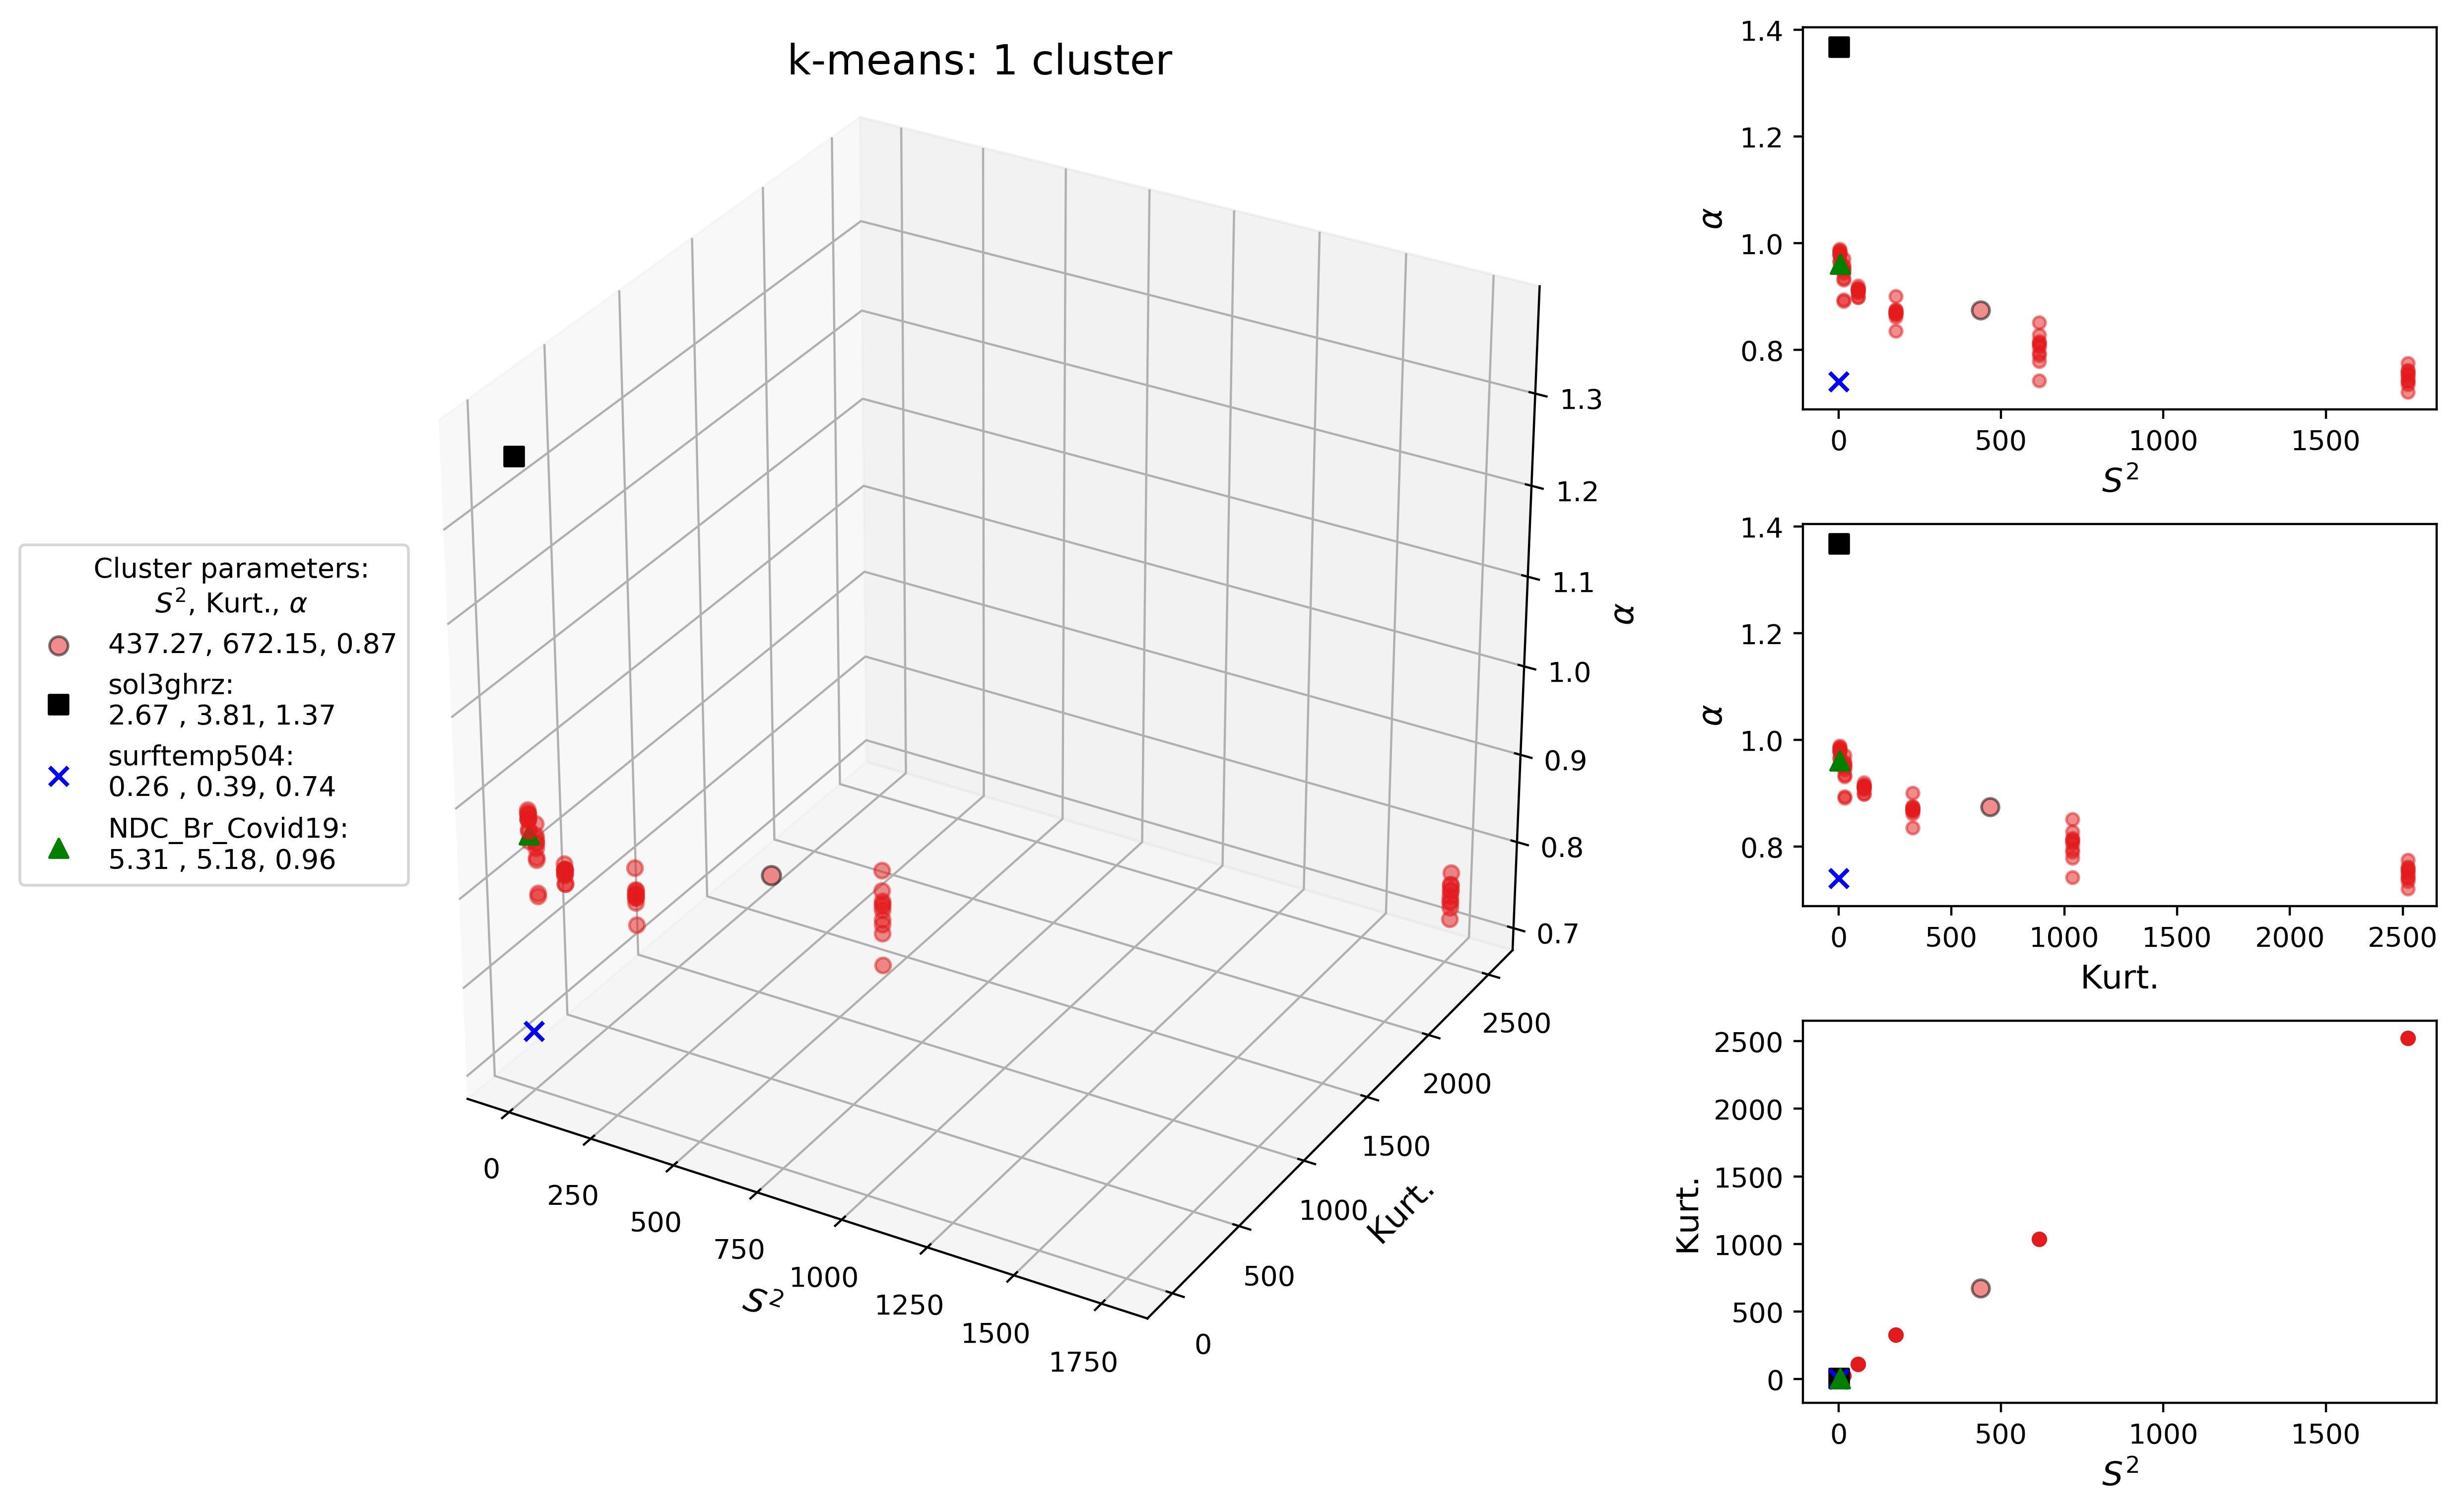
\includegraphics{Figuras/ex6/6_2/Exercicio6_2_grupo_pmnoise_DFA_cluster_1.jpg}}		
	\end{center}
	\vspace{-2mm}	% acrescentar o espaçamento vertical apropriado entre a borda inferior da figura e a legenda ou a fonte quando não há legenda (o valor pode ser negativo para subir)
	\legenda{Figura 6.2.3: Espaço skewness$^{2}$ x kurtosis x $\alpha$ do grupo pmnoise e a posição relativa das três séries temporais deste exercício. A série \textit{NDC\_Br\_Covid19} foi a que mais se aproximou dos sinais deste grupo.}	% legenda - para deixar sem legenda usar comando \legenda{} (nunca deve-se comentar o comando \legenda)
	\label{ex6_fig3}
	%\FONTE{}	% fonte consultada (elemento obrigatório, mesmo que seja produção do próprio autor)
\end{figure}

%%%%%%%%%%%%%%%%%%%%%%%%%%%%%%%%%%%%%%% 6.3 %%%%%%%%%%%%%%%%%%%%%%%%%%%%%%%5%%
\clearpage
\subsection*{6.3}
\addcontentsline{toc}{section}{\protect\numberline{} 6.3}%

Os dois plots a seguir resultam da análise da série \textit{ST-OWS\_NDC\_Covid19} para todos os países. O número de clusters ideal foi selecionado de acordo com o método do cotovelo, e foi de três para os dois espaços de parâmetros deste exercício. O algoritmo utilizado foi o kmeans\_2D\_group\_flags.py, que agrupou cada país em seu respectivo cluster em arquivos .csv (identificados pelo centróide do grupo). Estes arquivos e demais plots se encontram na pasta deste exercício - \textbf{6.3}. 

\begin{figure}[ht!]
	%\caption{Série e histogramas.}
	\vspace{0mm}	% acrescentar o espaçamento vertical apropriado entre o título e a borda superior da figura
	\begin{center}
		\resizebox{15cm}{!}{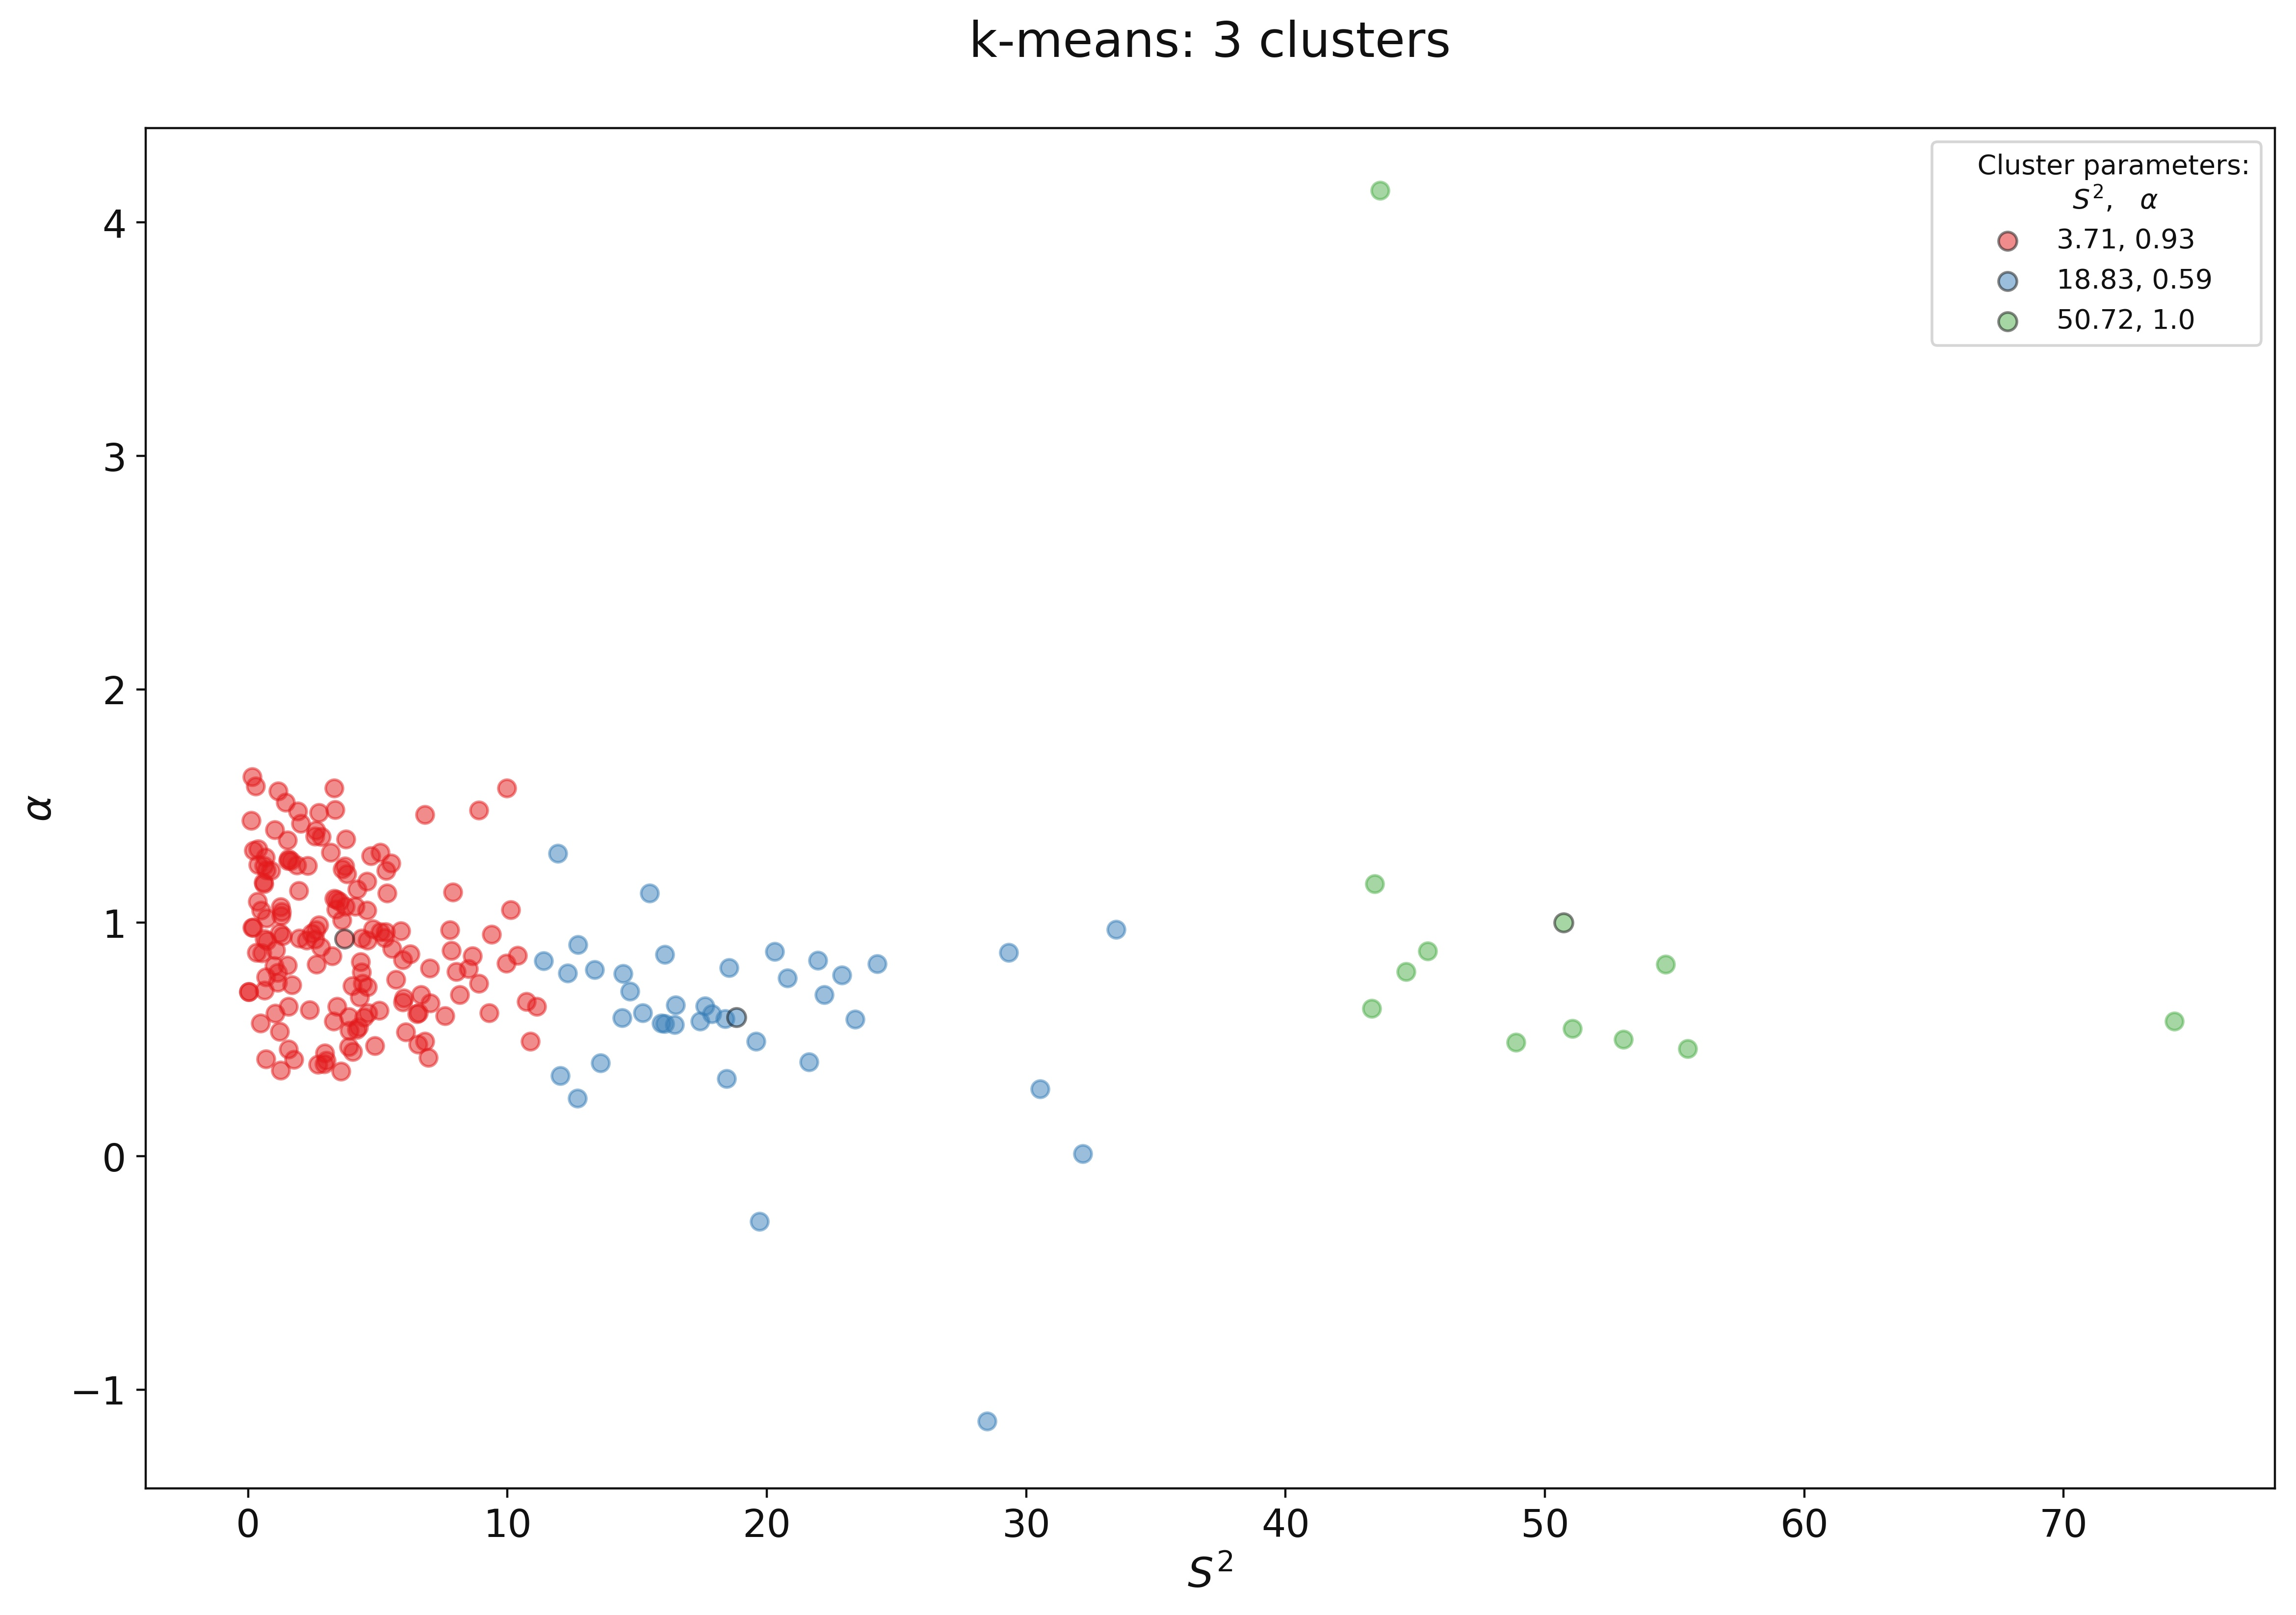
\includegraphics{Figuras/ex6/6_3/Exercicio6_3_S2vsAlfa_cluster_3.jpg}}		
	\end{center}
	\vspace{-2mm}	% acrescentar o espaçamento vertical apropriado entre a borda inferior da figura e a legenda ou a fonte quando não há legenda (o valor pode ser negativo para subir)
	\legenda{Figura 6.3.1: Resultado do agrupamento do número de casos diários de Covid19 para todos os países no espaço S$^{2}$ $\times$ $\alpha$.}	% legenda - para deixar sem legenda usar comando \legenda{} (nunca deve-se comentar o comando \legenda)
	\label{ex6_fig3}
	%\FONTE{}	% fonte consultada (elemento obrigatório, mesmo que seja produção do próprio autor)
\end{figure}

Nese exercício, os grupos de países no espaço S$^{2}$ x $\alpha$ se encontram nos seguintes arquivos: \textit{Exercicio6\_3\_S2vsAlfa\_cluster\_0\_x\_3.67\_y\_0.93\_flags.csv} (cluster vemelho), \textit{Exercicio6\_3\_S2vsAlfa\_cluster\_1\_x\_18.64\_y\_0.66\_flags.csv} (cluster azul) e \textit{Exercicio6\_3\_S2vsAlfa\_cluster\_2\_x\_53.82\_y\_1.04\_flags.csv} (cluster verde).

\clearpage

\begin{figure}[ht!]
	%\caption{Série e histogramas.}
	\vspace{0mm}	% acrescentar o espaçamento vertical apropriado entre o título e a borda superior da figura
	\begin{center}
		\resizebox{15cm}{!}{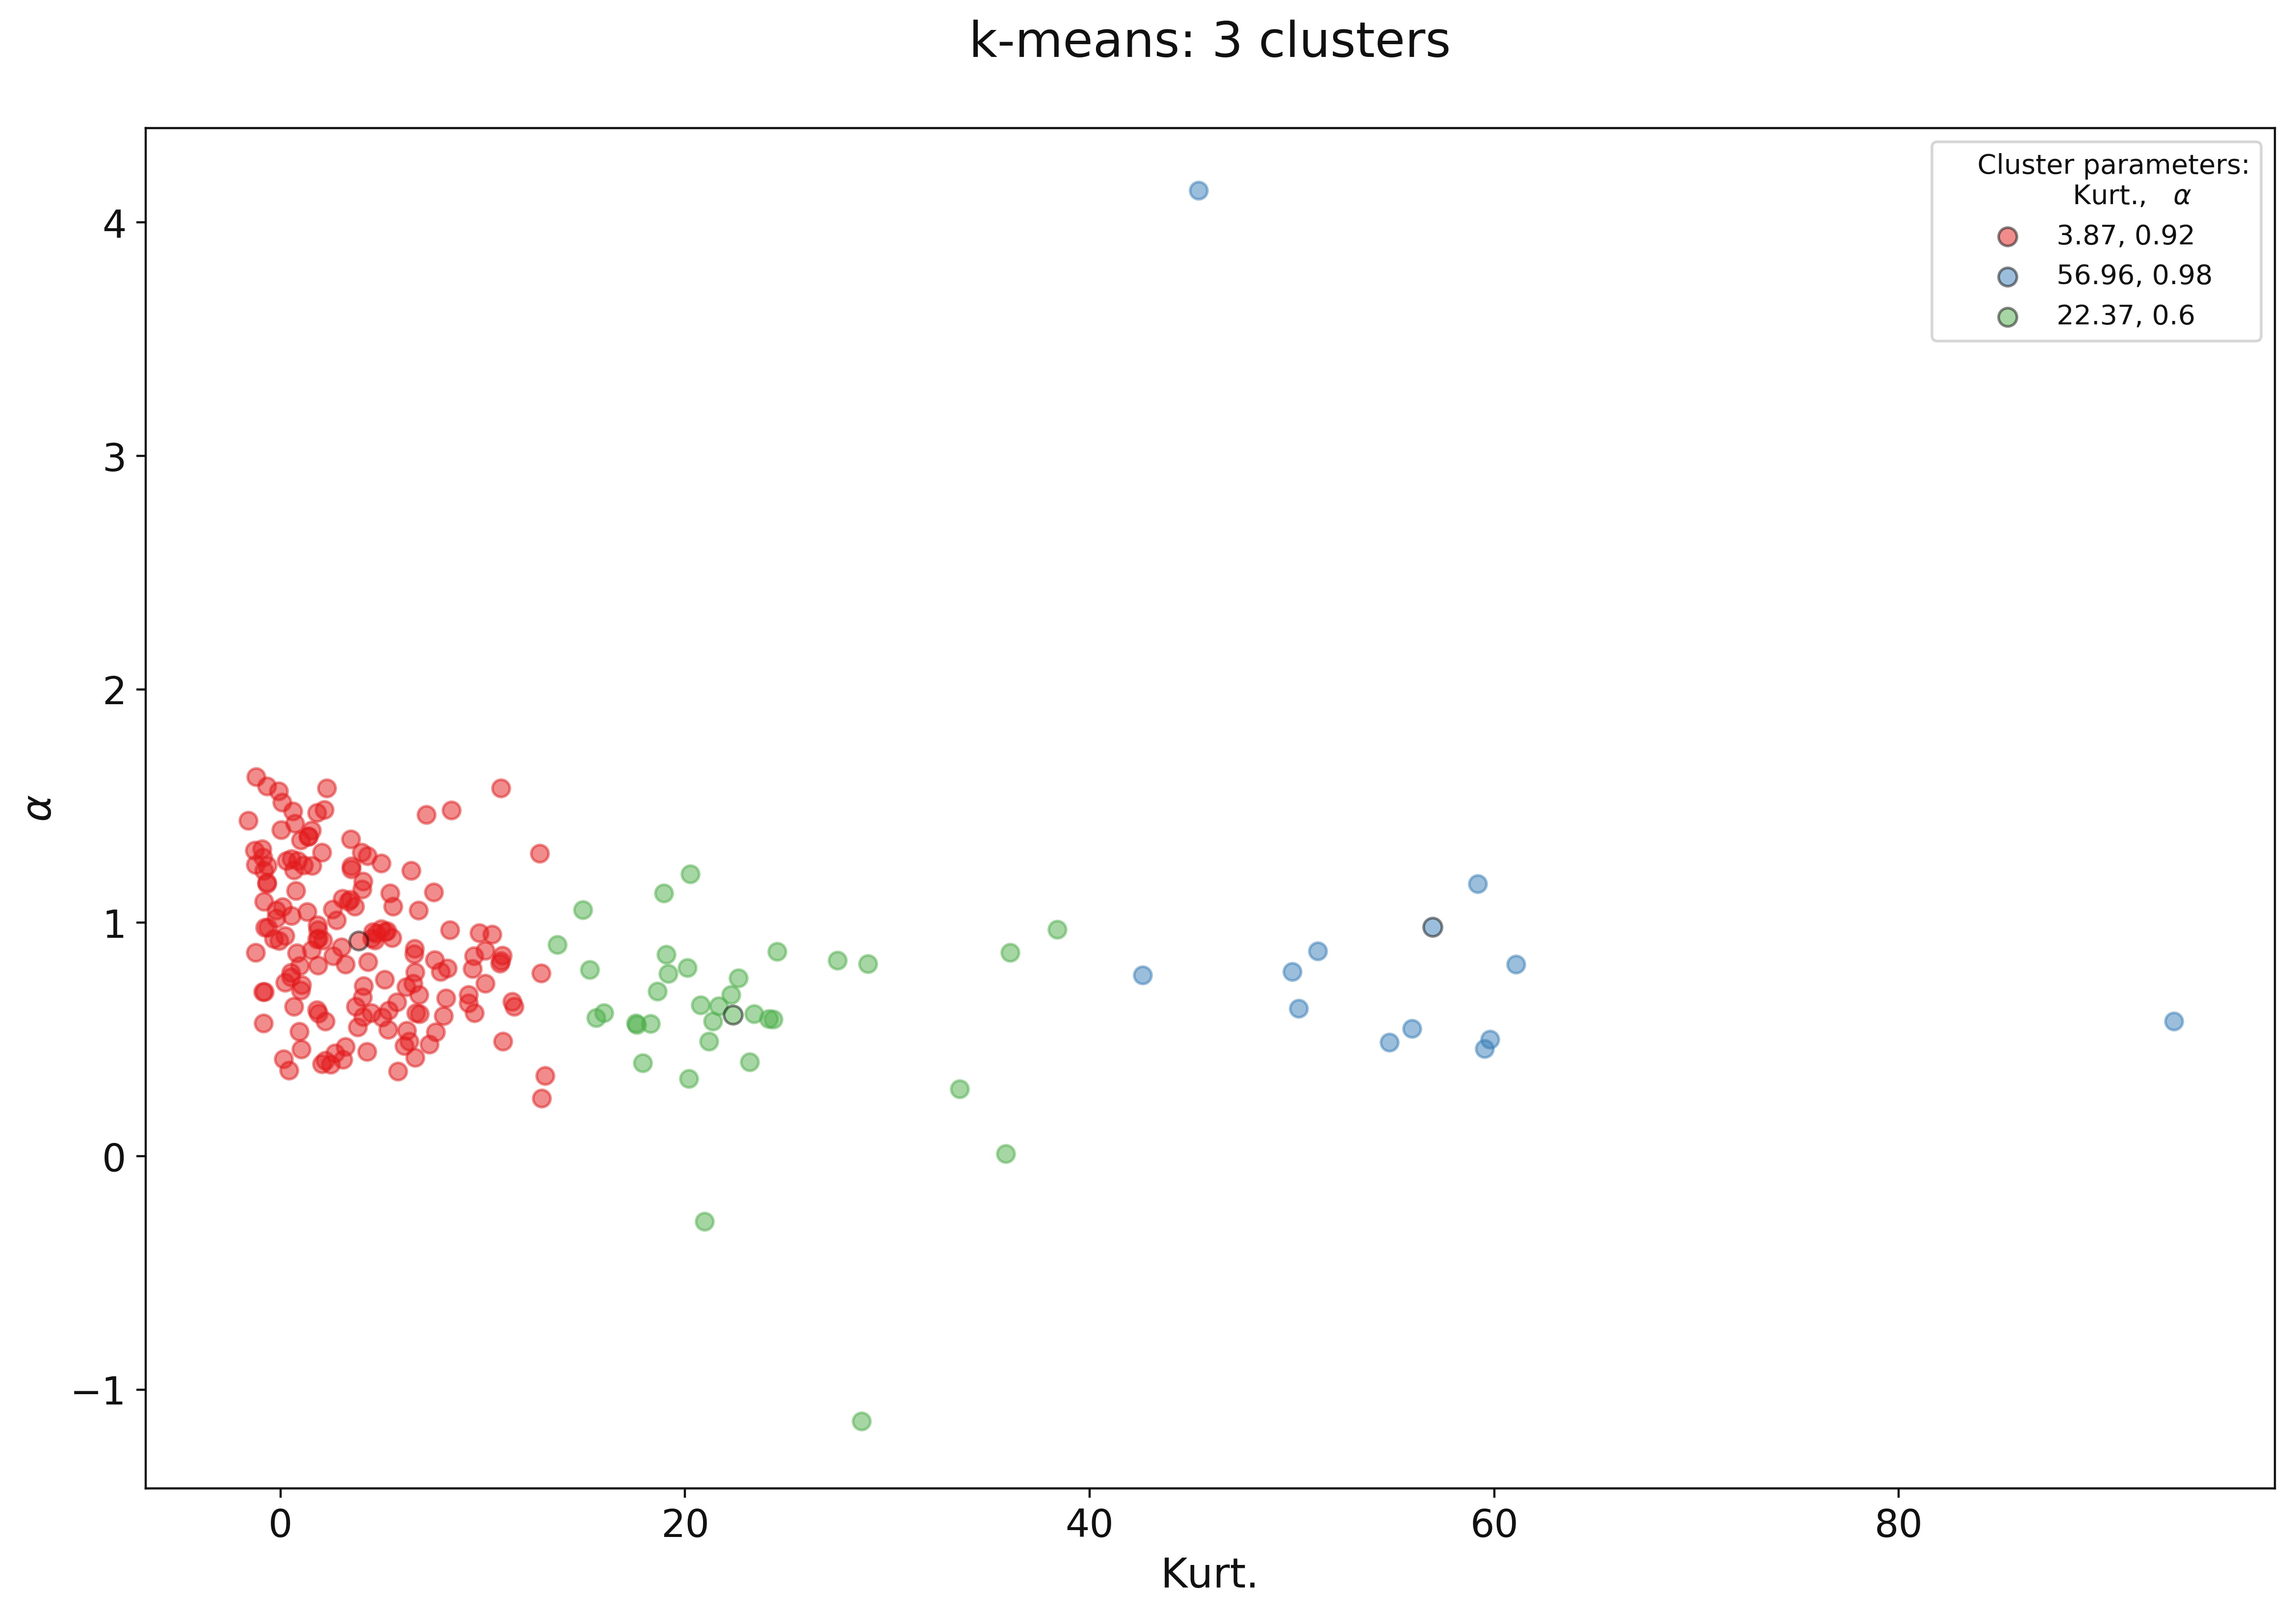
\includegraphics{Figuras/ex6/6_3/Exercicio6_3_KvsAlfa_cluster_3.jpg}}		
	\end{center}
	\vspace{-2mm}	% acrescentar o espaçamento vertical apropriado entre a borda inferior da figura e a legenda ou a fonte quando não há legenda (o valor pode ser negativo para subir)
	\legenda{Figura 6.3.2: Resultado do agrupamento do número de casos diários de Covid19 para todos os países no espaço K $\times$ $\alpha$.}	% legenda - para deixar sem legenda usar comando \legenda{} (nunca deve-se comentar o comando \legenda)
	\label{ex6_fig3}
	%\FONTE{}	% fonte consultada (elemento obrigatório, mesmo que seja produção do próprio autor)
\end{figure}

Nese exercício, os grupos de países no espaço K x $\alpha$ se encontram nos seguintes arquivos: \textit{Exercicio6\_3\_KvsAlfa\_cluster\_0\_x\_3.61\_y\_0.92\_flags.csv} (cluster vemelho), \textit{Exercicio6\_3\_KvsAlfa\_cluster\_1\_x\_58.83\_y\_1.02\_flags.csv} (cluster verde) e \textit{Exercicio6\_3\_KvsAlfa\_cluster\_2\_x\_20.72\_y\_0.66\_flags.csv} (cluster azul).